\documentclass[bsc,letterpaper,12pt]{csthesis}
%\documentclass[letterpaper,12pt,twoside]{csthesis} % para imprimir de lado y lado


\paperwidth = 21.6cm		% Tamaño de la hoja
\paperheight = 27.9cm

%Margenes horizontales
\hoffset = -2.54cm		% Se elimna el offset horizontal
\oddsidemargin = 4cm
\evensidemargin = 2cm
\textwidth = 15.6cm

%Margenes verticales
\voffset = -2.54cm
\topmargin = 3cm
\headheight = 0cm
\headsep = 0cm
\textheight = 21.9cm
\footskip = 1cm


\usepackage[spanish,USenglish]{babel}     % Idioma Capitulos y demas
\usepackage[utf8]{inputenc}
\usepackage{lmodern}
\usepackage[T1]{fontenc}
\usepackage{cc/CreativeCommons}  %Licencia

\usepackage{listings} % Ingresar Codigo Fuente
\usepackage{verbatim}
\usepackage{moreverb}
\let\verbatiminput=\verbatimtabinput
\def\verbatimtabsize{8}  % Tabulación en verbatim

% Paquete para el manejo de hipervinculos
\usepackage[b5paper, breaklinks=true, pdfborder={0 0 0},colorlinks=false,pageanchor=true, 
plainpages=false,bookmarksopen=true,bookmarksopenlevel=3, hyperfootnotes=false]{hyperref}

% Paquete para el manejo de tablas
\usepackage{supertabular}

% Paquetes para simbolos
%\usepackage{mathcomp}
\usepackage{latexsym}
\usepackage{pifont}
\usepackage{amsfonts}
\usepackage{amssymb}
\usepackage{wasysym}
\usepackage{colortbl}
\usepackage{multicol} 
\usepackage{booktabs}
\usepackage{multirow}
\usepackage{algorithmic}
\usepackage[Algoritmo]{algorithm}
\usepackage{subfigure}


% Manejo de imagenes PDF y EPS
\newif\ifpdf
\ifx\pdfoutput\undefined
\pdffalse % we are not running PDFLaTeX
\else
\pdfoutput=1 % we are running PDFLaTeX
\pdftrue
\fi

\ifpdf
\usepackage[pdftex]{graphicx}
\else
\usepackage{graphicx}
\fi

\ifpdf
\DeclareGraphicsExtensions{.pdf, .jpg, .tif}
\else
\DeclareGraphicsExtensions{.eps, .jpg}
\fi

% Sangria de comienzo de parrafo
\setlength{\parindent}{0cm}
% Espacio vertical entre dos parrfos
\setlength{\parskip}{0.3cm}

% Definir el nombre de listas
\addto\captionsspanish{%
  \def\prefacename{Prefacio}%
  \def\refname{REFERENCIAS}%
  \def\abstractname{RESUMEN}%
  \def\bibname{REFERENCIAS}%
  \def\chaptername{Cap\'{\i}tulo}%
  \def\appendixname{Anexo}%
  \def\listfigurename{Lista de figuras}%
  \def\listtablename{Lista de cuadros}%
  \def\indexname{\'Indice alfab\'etico}%
  \def\figurename{Figura}%
  \def\tablename{Tabla}%
  \def\partname{Parte}%
  \def\enclname{Adjunto}%
  \def\ccname{Copia a}%
  \def\headtoname{A}%
  \def\pagename{P\'agina}%
  \def\seename{v\'ease}%
  \def\alsoname{v\'ease tambi\'en}%
  \def\proofname{Demostraci\'on}%
  \def\glossaryname{Glosario}}
  \addto\captionsspanish{\def\contentsname{CONTENIDO}}
  
\addto\captionsUSenglish{
  \def\abstractname{ABSTRACT}%
}  

%para rotar tablas  
\usepackage{rotating}



%partir palabras
\hyphenation{di-fe-ren-cia pro-pues-to pro-ble-mas po-pu-la-res cons-truccio-nes ne-ce-sa-ria-men-te}

% Inico del documento
\begin{document}
\selectlanguage{spanish}
\pagestyle{empty}% Sin número de página
%%% PORTADA


\thispagestyle{empty}
\vspace*{1 mm}
\begin{center}{\centering \large VISUALIZACIÓN DEL POTENCIAL DE RADIACIÓN SOLAR EN EL DEPARTAMENTO DE NARIÑO UTILIZANDO SERIES DE TIEMPO A PARTIR DE IMÁGENES SATELITALES}
\end{center}

\vspace{2.5cm}

\begin{center}{\large BAYRON ANTONIO CHAMPUTIZ MARTINEZ}
\end{center}

\vspace{1.5cm}

\begin{figure}[!h]
\begin{center}

\includegraphics[scale=1]{pictures/udenar.eps}%logo of your university
\end{center}
\end{figure}

\vspace{3.5cm}

\begin{center}{\large UNIVERSIDAD DE NARIÑO\\
FACULTAD DE INGENIERÍA\\
DEPARTAMENTO DE SISTEMAS\\
PROGRAMA DE INGENIERÍA DE SISTEMAS\\
SAN JUAN DE PASTO\\
2016}
\end{center}



\pagebreak

\newpage

% CONTRAPORTADA

\thispagestyle{empty}

\vspace*{1 mm}
\begin{center}{\centering \large VISUALIZACIÓN DEL POTENCIAL DE RADIACIÓN SOLAR EN EL DEPARTAMENTO DE NARIÑO UTILIZANDO SERIES DE TIEMPO A PARTIR DE IMÁGENES SATELITALES}
\end{center}

\vspace{2.5cm}

\begin{center}{\large BAYRON ANTONIO CHAMPUTIZ MARTINEZ}
\end{center}

\vspace{1cm}

\begin{center}
{\large TRABAJO DE GRADO PRESENTADO COMO REQUISITO PARCIAL PARA OPTAR AL TÍTULO DE  
{INGENIERO DE SISTEMAS}}
\end{center}

\vspace{1cm}

\begin{center}
{\large DIRECTOR:  OMAR ERNESTO CABRERA ROSERO, ING.} 
\end{center}

\vspace{4.5cm}

\begin{center}{\large UNIVERSIDAD DE NARIÑO\\
FACULTAD DE INGENIERÍA\\
DEPARTAMENTO DE SISTEMAS\\
PROGRAMA DE INGENIERÍA DE SISTEMAS\\
SAN JUAN DE PASTO\\
2016}
\end{center}

\pagebreak

\chapter*{NOTA DE RESPONSABILIDAD}

``Las ideas y conclusiones aportadas en la tesis de grado, son 
responsabilidad exclusiva de sus autores''.

Articulo 1$\textordmasculine$ del acuerdo N$\textordmasculine$ 324 del 11 de octubre de 1966, 
emanado del 
Honorable Consejo Directivo de la Universidad de Nariño

``La Universidad de Nariño no se hace responsable de las opiniones o resultados obtenidos 
en el presente trabajo y para su publicación priman las normas sobre el derecho de autor''

Artículo 13, Acuerdo N. 005 de 2010 emanado del Honorable Consejo Académico.

\newpage
\vspace*{1 mm}
\begin{flushright}
Nota de aceptación:\linebreak \linebreak \linebreak 

\underline{\hspace{8cm}}\linebreak \linebreak
\underline{\hspace{8cm}}\linebreak \linebreak
\underline{\hspace{8cm}}\linebreak \linebreak
\underline{\hspace{8cm}}

\vspace{1cm}
\underline{\hspace{8cm}}\\
Firma del presidente del jurado \linebreak \linebreak \linebreak \linebreak \linebreak 

\underline{\hspace{8cm}}\\
Firma del jurado \linebreak \linebreak 

\vspace{1cm}
\underline{\hspace{8cm}}\\
Firma del jurado

\end{flushright}


\vspace{1cm}
San Juan de Pasto, 2016 


\newpage
\pagestyle{empty}
%\CCbysaInfo	%Licencia  Attribution-ShareAlike 3.0
%\CCbyInfo	%Creative Commons Attribution 3.0
%\CCbyndInfo	%Creative Commons Attribution-No-Derivs 3.0
\CCbyncInfo	%Creative Commons Attribution-Non-Commercial 3.0
%\CCbyncsaInfo	%Creative Commons Attribution-Non-Commercial-ShareAlike 3.0
%\CCbyncndInfo	%Creative Commons Attribution-Non-Commercial-NoDerivs 3.0



\chapter*{}
%pagenumbering{Roman} % para comenzar la numeracion de paginas en numeros romanos
\begin{flushright}
\textit{Dedicado a: \\
A mi madre Maria Martinez y a mi padre José Champutis,
por todo el apoyo que fué brindado durante el transcurso de mi carrera,
gracias por inculcarme valores que me permiten tener armonía en mi entorno social, 
por aconsejarme en de la mejor manera y estar presente en todas las dificultades.}

\textit{A mis compañeros de estudio que me brindaron ayuda incondicional,
fortaleza en momentos de debilidad,consejo y orientación en momentos de incertidumbre.}

\textit{A todos los profesores que contribuyeron con conocimientos, enseñanzas,
 consejos y experiencias en los momentos necesarios y oportunos, en especial a los docentes Andres Oswaldo Calderon y Jimmy Mateo Guerrero.\\}
\textit{A mi asesor, amigo y compañero Ing. Omar Ernesto Cabrera por brindar las experiencias y conocimiento pertinentes en la etapa de investigación.}


\textit{Al Grupo de Investigación en Ingeniería Eléctrica y Electrónica (GIIEE) por acogerme y brindarme apoyo pertinente en el transcurso de la investigación.
\\
\textbf{\\``Bayron Antonio Champutiz Martinez''}}
\end{flushright}


\chapter*{AGRADECIMIENTOS} % si no queremos que añada la palabra "Capitulo"

El presente trabajo de grado está dedicado a mis padres por el apoyo a mi formación personal y profesional, 
por confiar siempre en mis cualidades y entregarme su apoyo incondicional,
gracias porque siempre están presentes para apoyarme en cualquier dificultad.

Agradezco a Dios, por darme la fe y la fuerza necesaria en todo momento y permitirme creer que es posible culminar con éxito cualquier meta 
a pesar que existen momentos que se pueden tornar difíciles.


También está dedicado a todos aquellos amigos incondicionales que compartieron un momento de sus vidas conmigo y siempre me seguirán apoyando sin importar las circunstancias.
 
\selectlanguage{spanish}

\begin{abstract}
 Actualmente el la revolución de fuentes energéticas y los cambios acelerados 
 de las condiciones climáticas obliga a las naciones a plantear un cambio a los 
 enfoques de generación de energía, para esta serie de cambios se requiere un 
 análisis de todas y cada una de las fuentes de energía renovables y en varias 
 situaciones es pertinente resaltar las condiciones necesarias para optimizar el aprovechamiento del potencial energético. 
 La actual investigación se centró en la  construcción de una serie de tiempo en radiación 
 solar presente en el departamento de Nariño, con el objetivo principal de brindar 
 apoyo en el estudio de indicadores para radiación solar en el proyecto “Análisis de oportunidades energéticas con 
 fuentes alternativas en el departamento de Nariño”, 
 proyecto que realiza un estudio de diversas fuentes de energía presentes en el departamento.

 La investigación comprende descargar, procesar y analizar 11 años de imágenes satelitales 
 brindadas por el sensor MODIS y 15 años de imágenes satelitales 
 brindadas por el sensor Landsat, almacenar en una base de datos las bandas necesarias para 
 la identificación de radiación solar, aplicar modelos para la construcción de mapas de radiación solar, series de tiempo de radiación solar y nubosidad, realizar un análisis enfocado 
 en la detección de patrones, análisis del comportamiento de la 
 radiación solar y nubosidad en el departamento de Nariño.

Adicionalmente se pretende establecer y compartir los diferentes tipos de información y 
metodologías aplicadas a los interesados en la temática enfocada en el procesamiento y 
análisis de imágenes satelitales MODIS y LandSat.\\

\textbf{Palabras clave:}  MODIS, LandSat, detección de patrones, detección de nubes, análisis de regresión,
 series de tiempo, patrones secuenciales.
\end{abstract}


\selectlanguage{USenglish}

\begin{abstract}
Currently the Revolution energy sources and the rapid changes of weather 
conditions forces nations to propose a change to the approaches of power generation,
for this series of changes required an analysis of each and every one of the sources of renewable energy;
in some situations it is relevant to note the conditions to optimize use of the energy potential.
Current research focuses on the construction of a time series of solar radiation 
present in the department of Nariño, with the main objective of supporting indicators
in the study of solar radiation in the “Análisis de oportunidades energéticas con 
 fuentes alternativas en el departamento de Nariño” project; This project is conducting a study of 
various sources of energy present in the department.\\

The research includes download, process and analyze 11 years of satellite images provided by MODIS sensor and 15 years of 
satellite images provided by Landsat sensor,
storing in a database the necessary bands for detecting solar radiation, making a focused pattern detection analysis,
to visualize the behavior of solar radiation on the department of Nariño.\\

Additionally it is to establish and share different types of information and
methodologies applied to those interested in the topic focused on the processing and analysis
of MODIS satellite image.


\textbf{Keywords:} MODIS, LandSat,, pattern detection, detection of clouds, regression analysis,
Time series, sequential patterns.
\end{abstract}
 

\selectlanguage{spanish}
\tableofcontents
\chapter*{ACRÓNIMOS}
 
\begin{description}
 \item [CAD] Computer Aided Design
 \item [DBMS] Database Management System
 \item [GIS] Geographic Information System
 \item [LCM] Linear time Closed itemset Miner
 \item [MOD] Moving Objects Databases
 \item [MOD09GA] The MODIS Surface Reflectance products
 \item [MODIS] Moderate-Resolution Imaging Spectroradiometer
 \item [MPS] Minería de Patrones Secuenciales
 \item [RN] Redes Neuronales
 \item [KDD] Knowledge Discovery in Databases
 
\end{description}

\chapter*{INTRODUCCIÓN}
\addcontentsline{toc}{chapter}{INTRODUCCIÓN}
 
Países como Alemania, España, Japón, Estado Unidos, Italia son las potencias mundiales 
en la generación de energía renovable mediante el uso de energía solar,  este tipo de 
fuente de energía limpia ha adquirido gran importancia en el entorno investigativo en los 
últimos años y han surgido grandes expectativas para el futuro. 

Cada año el sol arroja 4000 veces más energía que la que se consume, lo que demuestra 
que esta fuente energética está aún infravalorada y desaprovechada  en relación a sus potenciales energéticos; 
la implementación para esta fuente energética es posible si un territorio cuenta una buena posición 
geográfica, economía sostenible y fenómenos climáticos regulados, estas condiciones favorables para la energía a base 
de paneles solares o energía térmica se encuentran presentes en muchas regiones de América Central y América del Sur,
 como ventaja adicional la energía solar puede aprovecharse directamente o almacenarse para un consumo posterior y no tiene riesgo de agotarse.

A pesar de que el Colombia cuenta con las condiciones ideales para producir energía solar, 
aún existen regiones del territorio colombiano donde la sociedad aún esta destinada a vivir sin energía eléctrica, un caso 
particular es el territorio nariñense donde varias poblaciones costeras cuentan con la radiación solar
necesaria para abastecer el consumo requerido en esa región y adicionalmente vender la energía sobrante a poblaciones cercanas, y sin embargo
no se ha realizado un estudio enfocado en el aprovechamiento de la energía a base de radiación solar presente en el departamento de Nariño; es necesario un
estudio para el comportamiento de la radiación solar en lugares con potencial energético, un análisis del comportamiento de fenómenos 
climáticos en zonas del departamento de Nariño, esta y más información que es de gran importancia para la implementación 
de generadores a base de energía solar.

\textbf{Planteamiento del problema}

El clima colombiano posee grandes características para implementación de plantas de energía renovable debido a 
la ubicación geográfica en la zona ecuatorial, características geográficas que favorecen la presencia del clima tropical 
y una temperatura uniforme la mayor parte del año. La posición estratégica de Colombia en la zona tropical genera 
muchos beneficios a la gran mayoría de departamentos, ocasionando que los territorios reciban una mayor proporción 
de energía que el sol le transfiere a la Tierra. 

El departamento de Nariño hereda la diversidad de climas presentes en el territorio colombiano, en esta zona el clima es más 
estable y menos variable respecto a cambios en los fenómenos climáticos que obedecen a las posición de una zona o altitud 
donde se encuentra un lugar determinado, la información referente al comportamiento de estas característica son de gran 
beneficio para aprovechar de forma óptima las diferentes fuentes de energía renovable. El proyecto “Análisis de oportunidades energéticas con fuentes alternativas 
en el departamento de Nariño” busca aprovechar los recursos naturales disponibles en este departamento con el objetivo inicial de
estudiar y analizar las fuentes de energías biomasa, hidráulica, viento y solar que se encuentran presentes dentro del departamento; 
el presente proyecto de investigación busca realizar el estudio previo para identificar las zonas con posible potencial solar para generar 
energía, la radiación solar es una fuente renovable utilizada mucho tiempo atrás por paises desarrollados, y actualmente  el manejo de esta 
fuente energética es una tendencia de las grandes potencias mundiales para mejorar la economía y mitigar los efectos de agentes contaminates.

La información que provee el IDEAM no permite tener gran certeza en los datos de radiación para una zona determinada, esto se debe a que cuenta con 
un número reducido de estaciones y es imposible tratar de generalizar datos aproximados para un territorio con grandes variaciones en su terreno, por este motivo
se puede decir que en la actualidad el departamento de Nariño no cuenta con un estudio preciso en información de radiación solar,información que podría 
ser usada y aprovechada para plantas energéticas a base de las fuentes de energía renovable. Tener un registro histórico de 
la información climatológica es muy importante debido a que se puede hacer una predicción del comportamiento de fenómenos climáticos como nubes, viento, 
características de la vegetación, radiación solar, precipitaciones o datos que permitan la identificación de zonas con potencial 
energético en una zona específica del territorio nariñense. El actual proyecto de investigación se enfoca 
en el estudio de radiación solar, mediante la construcción de una serie de tiempo de 11 años de información referente a 
radiación solar, comportamiento de la radiación en zonas determinadas y el comportamiento de nubes sobre el 
departamento de Nariño; actualmente la información referente a la cantidad de energía radiante que llega a la superficie del 
departamento en una época o tiempo determinado es difícil establecer y muy complejo de predecir; por este motivo el presente 
estudio resuelve esta carencia de información, la investigación radica en el procesamiento y análisis de imágenes 
satelitales  de libre acceso proveídas por el sensor MODIS y Landsat, imágenes que a partir de las características y propiedades
del sensor presenta determinado número de bandas con la capacidad de representar la medida de la gama de frecuencias capturada 
por el sensor, esta información representada en un formato determinado permite establecer características geográficas, hidrográficas, 
climáticas, vegetación, gases atmosféricos, radiación solar, precipitación y otro tipo información adicional del planeta
que se encuentra presentes en los últimos sensores activos. 

El estudio de energía solar mediante procesamiento y análisis de imágenes satelitales actualmente está 
apoyado por el uso de herramientas de libre acceso especializadas para realizar análisis de la información, aplicación de modelos
de regresión, construcción de series de tiempo, visualización del potencial energético a través de mapas de radiación solar 
y detección de patrones secuenciales en una serie de tiempo.

\textbf{Objetivo general}

Detectar patrones secuenciales que permitan predecir el comportamiento de fenómenos climáticos y su impacto en  áreas con potencial 
de radiación solar dentro del departamento de Nariño.


\textbf{Objetivos Específicos}

\begin{itemize}
 \item Construir series de tiempo de radiación solar dentro del área de estudio a partir del procesamiento de imágenes satelitales de libre acceso.
 \item Detectar la presencia de nubosidad en las imágenes satelitales obtenidas utilizando los algoritmos más pertinentes.
 \item Seleccionar y aplicar herramientas para la detección de patrones secuenciales.
 \item Generar un conjunto de datos que relacione la presencia de nubosidad en regiones con potencial de radiación solar.
 \item Validar la relación de resultados obtenido mediante la comparación datos producto  del estudio con datos reales capturados con algunos sensores activos.
 \item Generar mapas y reportes que permitan visualizar la radiación solar presente en el departamento de Nariño.
\end{itemize}


\textbf{Organización del documento}

Este documento está organizado en 5 secciones, la primera sección abarca los fundamentos teóricos empleados en la investigación,
la sección 2 presenta la metodología utilizada para el desarrollo de la investigación, esta sección se desarrolla en las 
siguientes fases: a)la identificación y adquisición de imágenes satelitales, b)procesamiento y almacenamiento de la 
información, c)selección, aplicación del modelo de regresión y construcción de series de tiempo, d)mapas de radiación solar usando 
interpolación espacial, e)detección de patrones secuenciales, f)comportamiento de las nubes; la sección 3 contiene la información 
referente a la validación de la información, en la sección 4 se presentan las conclusiones y trabajos futuros 
y para finalizar se presenta referencias bibliográficas y los anexos correspondientes.
\chapter{FUNDAMENTOS TEÓRICOS}

\section{Series de tiempo}

Son una secuencia de observaciones refiriéndose a datos que se recopilan y registran en intervalos de tiempo regulares, 
la información se encuentra ordenada cronológicamente por un único identificador de secuencia tanto cronológico como posicional. 
El principal objetivo de la series de tiempo, es permitir el análisis de la información procesada para hacer un  pronóstico 
de los futuros eventos.

Los componentes más comunes en las series de dependen de  la variación y al sobreponerse o actuar en concierto, contribuyen a 
los cambios observados en un período de tiempo y dan a la serie su aspecto errático. Estos componentes son: 

\textbf{Tendencia secular}:
también denominada tendencia a largo plazo de una serie es por lo común el resultado de factores a largo plazo. 
En términos intuitivos, la tendencia de una serie de tiempo caracteriza el patrón gradual y consistente de las variaciones de la propia serie, que se consideran consecuencias de fuerzas persistentes que afectan el crecimiento o la reducción de la misma
\\
\textbf{Variación estacional}:
comprende la representación de la variabilidad en los datos debida a influencias de las estaciones. Esta variación corresponde a los movimientos de la serie que recurren año tras año en los mismos meses del año poco más o menos con la misma intensidad.
\\
\textbf{Tendencia lineal}: la tendencia de una serie viene dada por el movimiento general a largo plazo de la serie. La tendencia a 
largo plazo de muchas series con frecuencia se aproxima a una línea recta. Esta línea de tendencia muestra que algo aumenta o 
disminuye a un ritmo constante. El método que se utiliza para obtener la línea recta de mejor ajuste es el Método de Mínimos Cuadrados. 
\\
\textbf{Tendencia no lineal}: cuando la serie de tiempo presenta un comportamiento curvilíneo se dice que este comportamiento es no lineal. 
Dentro de las tendencias no lineales que pueden presentarse en una serie se encuentran, la polinomial, logarítmica, exponencial y potencial, entre otras.



\section{Bases de Datos Espacio-Temporales}

Dos campos que han surgido a mediados y finales de la década de 1980 son las  bases de datos espaciales y bases de
datos temporales las cuales se han convertido, en cierto modo como  las precursoras de las bases de datos
espacio-temporales.


\textbf{Base de datos espaciales} 

Las bases de datos espaciales tratan del eficiente almacenamiento y la recuperación de objetos en
el espacio que tienen identidad y extensión bien definidas, ubicaciones, así como ciertas relaciones geométricas
y / o topológica entre ellas, debido al desarrollo en campos de aplicación ( GIS, diseño VLSI, CAD) que necesita
tratar  con  grandes cantidades de entidades geométricas, geográficas o espaciales. Además de algunos estables y 
maduros prototipos basado en fundamentos algebraicos de tipo solido,   proveedores de sistemas gestores de bases de
datos comercial (DBMS) han ofrecido extensiones de sus productos, soportando tipos espaciales y operaciones
(Oracle Spatial, DB2 Spatial Extender, PostgresGIS , Microsoft SQL Server, MySQL). Sin lugar a dudas, los 
resultados en bases de datos espaciales han impulsado varias líneas de investigación importantes en bases
de datos de objetos en movimiento (MOD), como por ejemplo: consultas  populares de MOD (rango, 
vecino mas cercano),  propiedades topológicas y relaciones entre tipos espaciales. \cite{yuzheng2011}


\textbf{Base de datos temporales}


Existen muchas aplicaciones de bases de datos, como por ejemplo, contabilidad, gestión de cartera, registros médicos
y gestión de inventario; información que varia en el tiempo. El centro de las bases de datos temporales se
diferencia por:

\begin{description}
 \item [Tiempo válido de un hecho,] es el tiempo en el cual un dato particular es recogido y se convierte en verdad
 hasta donde el mundo representado por la base de datos es referida, 
posiblemente abarque el pasado, el presente y el futuro. Sin embargo, el tiempo válido no puede ser 
conocido, o los registros no pueden ser relevantes para las aplicaciones soportadas por la base de datos
o en el caso que los modelos de base de datos del  mundo real puedan variar entre los diferentes mundos reales.

\item [Tiempo de transacción de un hecho,] es el tiempo que un hecho dado es el actual en la base de datos. 
El tiempo de transacción puede asociarse con diferentes entidades de bases de datos, como, por ejemplo,
objetos y valores que no son hechos, porque no pueden ser verdaderos o falsos en forma aislada. Por lo tanto, todas las entidades de la base de datos tiene un aspecto de  tiempo de transacción, que tiene
una duración: desde inserción (lógico) a la eliminación de una determinada entidad.
\end{description}


Capturar el tiempo variable utilizando los modelos de datos tradicionales y lenguajes de consulta
puede ser una actividad engorrosa y, como consecuencia, se necesitan construcciones que permitirán
capturar los tiempos válidos y operación de los hechos, lo que conduce a relaciones temporales. Además,
en los lenguajes de consulta se necesitan  extensiones sintácticas que permiten las operaciones de base
de datos en modelos temporales.  \cite{yuzheng2011}

\section{Técnicas de Regresión}

Permiten investigar y modelar la relación entre variables, la principal ventaja de la regresión es la descripción de los datos con el 
objetivo de resumir y ajustar un conjunto de datos. Adicionalmente es posible realizar una estimación de parámetros. Una vez 
seleccionado los modelos de regresión es necesario realizar un análisis y comparación de los diferentes modelos de regresión y 
chequear que tan bueno es un modelo ajustado respecto a otro. El resultado de este chequeo puede indicar si el modelo es razonable 
o si el ajuste original debe ser modificado.\\
\textbf{\\Selección de las variables del modelo}\\
Existen varios métodos para construir el modelo de regresión, es decir, para seleccionar de entre todas las variables que introducimos 
en el modelo, cuáles son las que necesitamos para explicarlo. El modelo de regresión se puede construir utilizando las siguientes técnicas \cite{regresionmodel}: 
\begin{itemize}
\item{\textbf{Técnica de pasos hacia adelante (Forward)} 
Consiste en ir introduciendo las variables en el modelo únicamente si cumplen una serie de condiciones hasta que no se pueda introducir 
ninguna más, hasta que ninguna cumpla la condición impuesta
}
\item{
\textbf{Técnica de pasos hacia atrás (Backward)}
Se introducen en el modelo todas las variables y se van suprimiendo si cumplen una serie de condiciones definidas a priori hasta 
que no se pueden eliminar más, es decir ninguna variable cumpla la condición impuesta.
}
\item{\textbf{Técnica por pasos (Stepwise)}
Combina los dos métodos anteriores, adelante y atrás introduciendo o eliminando variables del modelo si cumplen una serie de 
condiciones definidas a priori hasta que ninguna variable satisfaga ninguna de las condiciones expuestas de entrada o salida del modelo.
}
\item{\textbf{Técnica de introducir todas las variables obligatoriamente (Enter)}
Esta última técnica de selección de variables para construir el modelo de regresión, produce que el proceso de selección de las variables 
sea manual, partiendo de un modelo inicial, en el que se obliga a que entren todas las variables seleccionadas, se va evaluando qué variable 
es la que menos participa en él y se elimina, volviendo a construir un nuevo modelo de regresión aplicando la misma técnica, pero excluyendo 
la variable seleccionada y aplicando el mismo proceso de selección. Este proceso se repite reiteradamente hasta que se considere que el modelo 
obtenido es el que mejor se ajusta a las condiciones impuestas y que no se puede eliminar ninguna variable más de las que los componen.
}
\end{itemize}
\section{Redes Neuronales}
Se define redes neuronales a una nueva forma de computación inspirada en modelos biológicos, un modelo matemático compuesto
por un gran número de elementos procesales organizados en niveles, también se define redes neuronales a un sistema de computación compuesto 
por un gran número de elementos simples, elementos de procesos muy interconectados, los cuales procesan información por medio de su estado dinámico 
como respuesta a entradas externas o se puede definir las redes neuronales como redes interconectadas masivamente en paralelo de elementos simples y 
con organización jerárquica, las cuales intentan interactuar con los objetos del mundo real del mismo modo que lo hace el sistema nervioso 
biológicos~\ref{fig:rn}.
\begin{figure}[htb]
 \centering 
 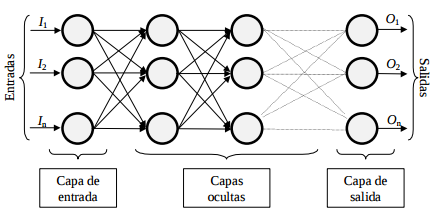
\includegraphics[scale=0.7]{pictures/rn.png}
 \caption{ un esquema de una red neuronal.} 
 \label{fig:rn}
\end{figure}
\newpage
Las redes neuronales presentan características como:
\begin{itemize}
 \item {\textbf{ Aprendizaje adaptativo}\\
 Las redes neuronales pueden aprender a diferenciar patrones mediante ejemplos y entrenamientos, no es necesario elaborar modelos a priori 
 ni necesidad de especificar funciones de distribución de probabilidad; las RN son sistemas dinámicos auto-adaptativos con la capacidad de 
 auto-ajuste de los elementos procesales (neuronas) que componen el sistema, son capaces de estar constantemente
cambiando para adaptarse a las nuevas condiciones; los enlaces ponderados de las neuronas se ajustan de manera que se obtengan ciertos 
resultados específicos. Una red neuronal no necesita un algoritmo para resolver un problema, ya que ella puede generar su propia distribución
de pesos en los enlaces mediante el aprendizaje. También existen redes que continúan aprendiendo a lo largo de su vida, después de completado 
su período de entrenamiento.
 }
\item {\textbf{ Auto-organización }\\
 Las redes neuronales emplean su capacidad de aprendizaje adaptativo para auto-organizar la información que reciben durante el aprendizaje 
 y/o la operación. Mientras que el aprendizaje es la modificación de cada elemento procesal, la auto-organización consiste en la modificación
 de la red neuronal completa para llevar a cabo un objetivo específico.
Cuando las redes neuronales se usan para reconocer ciertas clases de patrones,
ellas auto-organizan la información usada. Por ejemplo, la red llamada backpropagation,
creará su propia representación característica, mediante la cual puede reconocer ciertos
patrones.Esta auto-organización provoca la generalización: facultad de las redes
neuronales de responder apropiadamente cuando se les presentan datos o situaciones a
las que no había sido expuesta anteriormente. El sistema puede generalizar la entrada
para obtener una respuesta. 

Esta característica es muy importante cuando se tiene que
solucionar problemas en los cuales la información de entrada no es muy clara; además
permite que el sistema dé una solución, incluso cuando la información de entrada está
especificada de forma incompleta. 
 } 
 \item {\textbf{ Tolerancia a fallos }\\
 Las redes neuronales fueron los primeros métodos computacionales con la capacidad inherente de tolerancia a fallos. Comparados con los sistemas 
 computacionales tradicionales, los cuales pierden su funcionalidad cuando sufren un pequeño error de memoria, en las redes neuronales, si se 
 produce un fallo en un número no muy grande de neuronas y aunque el comportamiento del sistema se ve influenciado, no sufre una caída repentina.
Hay dos aspectos distintos respecto a la tolerancia a fallos:
\begin{itemize}
\item Las redes pueden aprender a reconocer patrones con ruido, distorsionados o
incompletos. Esta es una tolerancia a fallos respecto a los datos.
\item Las redes pueden seguir realizando su función (con cierta degradación)
aunque se destruya parte de la red.
\end{itemize}
La razón por la que las redes neuronales son tolerantes a los fallos es que tienen
su información distribuida en las conexiones entre neuronas, existiendo cierto grado de
redundancia en este tipo de almacenamiento. La mayoría de los ordenadores
algorítmicos y sistemas de recuperación de datos almacenan cada pieza de información
en un espacio único, localizado y direccionable. En cambio, las redes neuronales
almacenan información no localizada. Por lo tanto, la mayoría de las interconexiones
entre los nodos de la red tendrán sus valores en función de los estímulos recibidos, y se
generará un patrón de salida que represente la información almacenada. 
 } 
 \item {\textbf{ Operación en tiempo real }\\
 Una de las mayores prioridades, casi en la totalidad de las áreas de aplicación, es
la necesidad de realizar procesos con datos de forma muy rápida. Las redes neuronales
se adaptan bien a esto debido a su implementación paralela. Para que la mayoría de las
redes puedan operar en un entorno de tiempo real, la necesidad de cambio en los pesos
de las conexiones o entrenamiento es mínimo.
 } 
 \item {\textbf{ Fácil inserción dentro de la tecnología existente. }\\
 Una red individual puede ser entrenada para desarrollar una única y bien
definida tarea (tareas complejas, que hagan múltiples selecciones de patrones,
requerirán sistemas de redes interconectadas). Con las herramientas computacionales
existentes (no del tipo PC), una red puede ser rápidamente entrenada,
comprobada, verificada y trasladada a una implementación hardware de bajo
coste. Por lo tanto, no se presentan dificultades para la inserción de redes
neuronales en aplicaciones específicas, por ejemplo de control, dentro de los
sistemas existentes. De esta manera, las redes neuronales se pueden utilizar para
mejorar sistemas en forma incremental y cada paso puede ser evaluado antes de
acometer un desarrollo más amplio \cite{pitarque2000redes}.
 }
\end{itemize}

Entre las propiedades de las RN que han llamado la atención de los estadísticos destacan las relativas a su buen rendimiento ante
problemas no lineales o datos con mucho «ruido», y el poderse utilizar independientemente del cumplimiento de los supuestos teóricos 
relativos a las técnicas estadísticas (y de ahí que se haya hablado de ellas como de «técnicas de distribución libre o no paramétricas»). 
Por ello las RN han sido aplicadas a problemas de tradición estadística como predicción y clasificación (a través de las
llamadas redes hetero-asociativas: perceptrón multicapa y redes de función base radial), reducción de la dimensionalidad (a través
de las llamadas redes auto-asociativas: Hopfield, Kohonen),series temporales, etc.\cite{pitarque1998redes}\cite{maneta2003aplicacion}\cite{rn2001giaiq}.

\section{Interpolación Espacial}

La interpolación espacial es el proceso de utilizar puntos con valores conocidos para estimar valores desconocidos en otros puntos. 
Por ejemplo, para realizar un mapa de precipitación (lluvia) para el país no se encontrarán suficientes estaciones meteorológicas distribuidas
uniformemente para cubrir toda la región. La interpolación espacial puede estimar las temperaturas en lugares que no tienen ese dato utilizando 
lecturas de temperatura conocida en estaciones meteorológicas cercanas~\ref{fig:is}. A este tipo de superficie interpolada con 
frecuencia se le llama una superficie estadística. Datos de elevación, precipitación, acumulación de nieve, tabla de agua y densidad de población 
son otros tipos de datos que pueden ser calculados utilizando la interpolación \cite{qgis2015online}.

Debido al alto costo y a los recursos limitados la recolección de los datos usualmente es llevada a cabo sólo en un número limitado 
de ubicaciones de puntos seleccionados. En un SIG, la interpolación de esos puntos puede ser aplicada para crear una superficie raster con 
estimaciones realizadas para todas las celdas del raster. Con el fin de generar un mapa continuo, por ejemplo, un mapa de elevaciones digitales de 
los puntos de elevación medidos con un dispositivo GPS, se debe utilizar un método de interpolación adecuado para estimar de manera óptima los valores 
en aquellas ubicaciones en donde no fueron tomadas muestras o mediciones. Los resultados del análisis de interpolación pueden entonces ser utilizados 
para análisis que cubran el área completa y para el modelado.

\begin{figure}[htbp]
 \centering 
 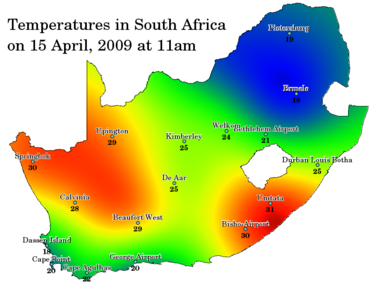
\includegraphics[width=0.6\textwidth]{pictures/is.png}
 \caption{Mapa de temperaturas interpolado de estaciones.}
 \label{fig:is}
\end{figure}
\textbf{Metodos de Interpolación}\bigskip

\textbf{Método Trend Surface}: es un método analítico, global e inexacto a partir de puntos. Este
método se utiliza para separar y describir determinados componentes de variación presentes
en los datos, facilitando su interpretación, puesto que cada una de las observaciones puede ser
considerada como resultado de la adición de un componente regional o de tendencia y un
componente local. Asimismo, considera la autocorelación de la variable.
Ajustándose la variable Z a una ecuación de regresión cuyas variables explicativas son X e Y
de los puntos muestrales. Proporciona una descripción sintética de la superficie ondulada que
se está tratando y de la variación espacial de la variable temática, facilitando un método para
estimar el valor de Z en un punto no muestral cuyas coordenadas X e Y sean conocidas Figura~\ref{fig:m1}.
\begin{figure}[htb]
 \centering 
 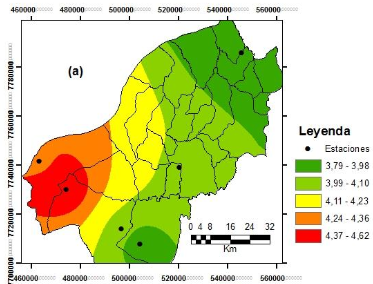
\includegraphics[width=0.47\textwidth]{pictures/a.png}
 \caption{Interpolación con el método Trend Surface\cite{models2013}}
 \label{fig:m1}
\end{figure}

\textbf{Método Moving average}: es un método directo, local, a partir de puntos, puede ser exacto
o no según el factor de ponderación. Se aplica para un gran conjunto de datos. Extrae
tendencias intermedias de un número mínimo de puntos definidos dentro de una Search
Elipse, asociada a cada uno de los puntos del grid. El valor final de cada uno de los puntos del
grid es igual a la media aritmética de todos los puntos vecinos identificados. Si dentro de la
Search elipse no hay un número mínimo de puntos definidos para el cálculo, el área estará en
blanco Figura~\ref{fig:m2}.
\begin{figure}[htb]
 \centering 
 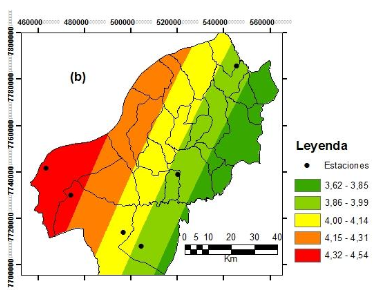
\includegraphics[width=0.47\textwidth]{pictures/b.png}
 \caption{Interpolación con el método Moving Average\cite{models2013}}
 \label{fig:m2}
\end{figure}

\textbf{Método Kriging}: es un método analítico, donde la función de interpolación depende de la
autocorelación espacial de la variable, que se representa en variogramas. Utiliza datos
tabulares y su posición geográfica para el cálculo de las interpolaciones. Utilizando el
principio de la primera ley geográfica de Tobler, que dice que las unidades de análisis más
próximas entre si son mas similares que las unidades más lejanas, el kriging utiliza funciones
matemáticas para añadir más peso en las posiciones más cercanas a los puntos de muestreo y
menores pesos en posiciones más distantes, y así crear nuevos puntos interpolados basados en
estas combinaciones lineares de datos. Además se está basado en optimizar funciones usando
autocorelación espacial Figura~\ref{fig:m3}.
\begin{figure}[htb]
 \centering 
 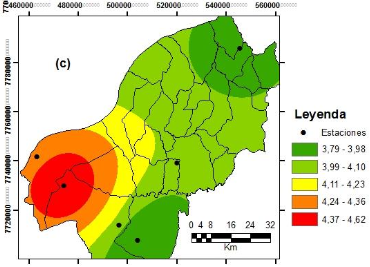
\includegraphics[width=0.5\textwidth]{pictures/c.png}
 \caption{Interpolación con el método Kriging \cite{models2013}}
 \label{fig:m3}
\end{figure}

\section{Minería de Datos}
El descubrimiento de conocimiento en bases de datos (KDD) se define como el proceso de identificar patrones significativos 
en los datos que sean válidos, novedosos, potencialmente útiles y comprensibles para un usuario. El proceso global consiste 
en transformar información de bajo nivel en conocimiento de alto nivel \cite{riquelme2006mineria}. El proceso KDD es interactivo e iterativo conteniendo
los siguientes pasos:
\begin{enumerate}
 \item \textbf{Comprender el dominio de aplicación:} este paso incluye el conocimiento relevante previo y las metas de la aplicación.
\item \textbf{Extraer la base de datos objetivo:} recogida de los datos, evaluar la calidad de los datos y utilizar análisis exploratorio de los datos para
familiarizarse con ellos.
\item \textbf{Preparar los datos:} incluye limpieza, transformación, integración y reducción de datos. Se intenta mejorar la calidad de los
datos a la vez que disminuir el tiempo requerido por el algoritmo de aprendizaje aplicado posteriormente.
\item \textbf{Minería de datos:} como se ha señalado anteriormente, este es la fase fundamental del proceso. Está constituido por una o más de
las siguientes funciones, clasificación, regresión, clustering, resumen, recuperación de imágenes, extracción de reglas, etc.
\item \textbf{Interpretación:} explicar los patrones descubiertos, así como la posibilidad de visualizarlos.
\end{enumerate}
A continuación se comentan brevemente las tareas más comunes en cualquier proceso de la minería de datos.
\begin{itemize}
 \item Clasificación: clasifica un dato dentro de una de las clases categóricas predefinidas. Responde a preguntas tales como, 
 ¿Cuál es el riesgo de conceder un crédito a este cliente? ¿Dado este nuevo paciente qué estado de la enfermedad indican sus análisis?
 \item Regresión: el propósito de este modelo es hacer corresponder un dato con un valor real de una variable. Responde a cuestiones como
¿Cuál es la previsión de ventas para el mes que viene? ¿De qué depende?
 \item Clustering: se refiere a la agrupación de registros, observaciones, o casos en clases de objetos similares. Un cluster es una colección
de registros que son similares entre sí, y distintos a los registros de otro cluster. ¿Cuántos tipos de clientes vienen a mi negocio? 
¿Qué perfiles de necesidades se dan en un cierto grupo de pacientes?
\item Generación de reglas: aquí se extraen o generan reglas de los datos. Estas reglas hacen referencia al descubrimiento de relaciones de 
asociación y dependencias funcionales entre los diferentes atributos.
\item Resumen o sumarización: estos modelos proporcionan una descripción compacta de un subconjunto de datos. ¿Cuáles son las
principales características de los datos?
\item Análisis de secuencias: se modelan patrones secuenciales, como análisis de series temporales, secuencias de genes, etc. El objetivo 
es modelar los estados del proceso, o extraer e informar de la desviación y tendencias en el tiempo. ¿El consumo de energía eléctrica de este 
mes es similar al del año pasado? Dados los niveles de contaminación atmosférica de la última semana cuál es la previsión para las próximas 24 horas.
\end{itemize}


\textbf{Patrones Frecuentes en Bases de Datos Tradicionales}

Patrones frecuentes son conjuntos de elementos, subsecuencias, o subestructuras que aparecen en un conjunto de datos con una
frecuencia no inferior a un umbral especificado por el usuario \cite{han2007frequent}. La cuestión de las modalidades 
interesantes desvelando en las bases de datos en diferentes contextos ha sido un tema de investigación
recurrente durante los últimos 15 años. Minería de datos general ha sido ampliamente reconocido como un
crítico campo por empresas de todo tipo. Como parte de los métodos de minería de datos, la tarea de aprendizaje 
de reglas de asociación han estudiado diferentes algoritmos de minería de patrones frecuente de identificar 
tendencias relevantes en los conjuntos de datos en diferentes disciplinas \cite{creighton2003mining}. 

Una de las áreas en las que las técnicas de aprendizaje de reglas de asociación y el patrón frecuente 
algoritmos de minería se han aplicado con más frecuencia en el análisis de datos y tendencias del
mercado en transacciones de clientes de grandes supermercados y tiendas \cite{agrawal1994fast}. Por lo general, esta técnica 
tiene dado el nombre del problema de la cesta de compras a pesar de que los métodos derivados de resolverlo
puede ser aplicado en diferentes contextos \cite{han2006data}.

\textbf{Minería de Patrones Secuenciales}

Sea DB un conjunto de registros (objetos), donde cada registro R consiste de tres
elementos de información:
\begin{itemize}
\item un identificador de registro object-id
\item un registro de tiempo timestamp
\item un conjunto A de atributos binarios
\end{itemize}
Un atributo a puede estar presente ’1’, o ausente ’0’. Si bien los algoritmos intentan encontrar secuencias de atributos
presentes, esta claro que su ausencia también brinda significativa información. Un atributo a presente es llamado
ítem i, y dentro del contexto de números, un ítem es una cupla (atributo, valor). Un conjunto de items
{i1, i2, · · · , ik} es denotado por I, donde I es un sub conjunto de A. Esto es una representación no ordenada. Una
secuencia s es una lista ordenada no vacía de los conjuntos de items s, denotado por hs1, s2, · · · , spi. Una nsecuencia
es una secuencia de n items o de tamaño n. Decimos entonces que R es un conjunto de registros que
contienen los atributo presente (o ítems) i. Gráficamente R(I) podría verse así como en la figura ~\ref{fig:atrib}.

\begin{figure}[htb]
  \centering 
  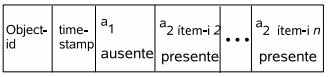
\includegraphics[scale=0.5]{pictures/atrib.png}
  \caption{Algunos Atributos Presentes o items.} 
  \label{fig:atrib}
\end{figure}

\textbf{Secuencia de datos} Una secuencia de datos hs1, s2, · · · , spi es una agrupación
ordenada de registros con atributos presentes iguales, similares o pertenecientes. La agrupación se ordena según los
datos de timestamp. \\
\textbf{Frecuencia de secuencias} Los grados de pertenencia se obtienen al evaluar la frecuencia
de ocurrencia de las secuencias freq(s) con distintos niveles. Algunos autores establecen un valor
de referencia o parámetro, por ejemplo minFreq, con el fin de decidir si una frecuencia es más o menos frecuente.\\

\textbf{LCM (Linear Time Closed Itemset Miner)}

El problema de LCM propuesto por \cite{uno2005lcm} se define de la siguiente manera.
Sea I un conjunto de elementos. Sea D una base de datos transaccional de tal manera que cada 
registro (llamada transacción) es un conjunto de elementos. La frecuencia de un conjunto de 
elementos es el número de transacciones, incluyendo el conjunto de elementos. Para un número dado t 
(llamado soporte), un conjunto de elementos se dice que es frecuente si su frecuencia es no menos de 
t. Un conjunto de elementos frecuente se llama máxima si está incluido en ningún otro conjunto de 
elementos frecuentes, y se llama cerrada si está incluido en ningún otro conjunto de elementos de la 
misma frecuencia. La tarea de LCM, es enumerar (sacar, o contar) todos los conjuntos de elementos 
frecuentes, todos los conjuntos de elementos frecuentes máximos, o todos los conjuntos de elementos 
frecuentes cerrados en una base de datos transaccional para un soporte dado.
\chapter{TRABAJOS RELACIONADOS}
Dada la creciente demanda por la generación y apropiamiento de las energías limpias, el estudio de alternativas energéticas basadas en paneles 
solares también ha venido en aumento. Sin embargo, un componente clave para la implementación de una solución de este tipo es analizar de antemano 
las posibles ubicaciones con mayor potencial de generación eléctrica a base de radiación solar. Diversos estudios han consolidado el uso de imágenes 
satelitales de libre acceso como herramientas fundamentales para este propósito. \cite{kaku2009creating} realizó la construcción de mapas solares de alta 
resolución comparando metodologías basadas en imágenes satelitales y modelamiento climático. Para estos modelos de radiación se contemplan condiciones 
propias del terreno como la latitud , el terreno,estación, hora del día y condicione atmosférica(nubes, polvo, polución, vapor de agua y efectos de la montaña)
\begin{figure}[ht]
  \centering 
  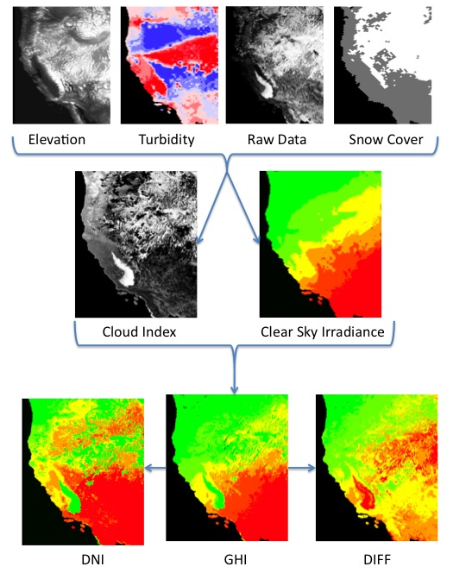
\includegraphics[scale=0.47]{pictures/ER1.png}
  \caption{Diagrama de flujo que representa el cálculo de los valores de irradiancia (Global Horizontal,Directa normal , y Difusa horizontal ) 
  de un área para un área, la fecha dada y ángulo cenital solar.} 
  \label{fig:er1}
\end{figure}
\newpage
\cite{hammer2003solarenergy} desarrolló el método HELIOSAT con el 
objetivo de estimar los niveles de radiación solar a partir de imágenes satelitales geoestacionarias, el método se encuentra implementado 
en un algoritmo que permite separar la irradiación de los componentes atmosférico de la irradiación en nubes para finalmente obtener la 
irradiación superficial.

\begin{figure}[htb]
  \centering 
  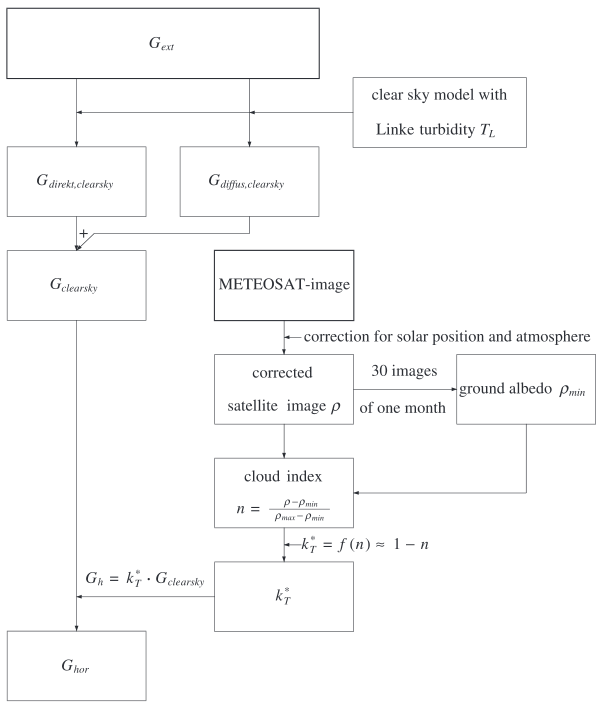
\includegraphics[scale=0.5]{pictures/ER2.png}
  \caption{Descripción general del método HELIOSAT.} 
  \label{fig:er2}
\end{figure}
\newpage
\cite{diagne2012solarirradiation} realiza una recopilación de métodos para la predicción de radiación solar también basados en imágenes por satélite o modelos climáticos, en este estudio 
se contempla la variación de la resolución espacial de la imágen satelital, tipos de sensores utilizados y la escala temporal.
\begin{figure}[htb]
  \centering 
  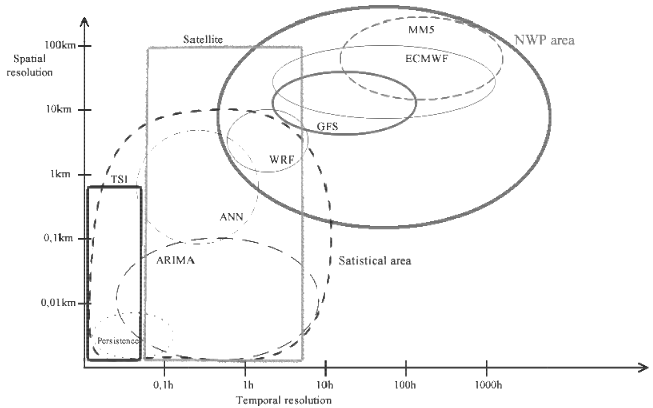
\includegraphics[scale=0.65]{pictures/ER3.png}
  \caption{Clasificación de modelos de predicción basados en resolución espacial de datos y resolución temporal.} 
  \label{fig:er3}
\end{figure}

\cite{wang2012shortterm} obtuvo gran éxito al proponer un nuevo modelo basado en redes neuronales apropiado para pronosticar el potencial solar a corto 
plazo bajo condiciones meteorológicas en constante cambio.

\begin{figure}[htb]
  \centering 
  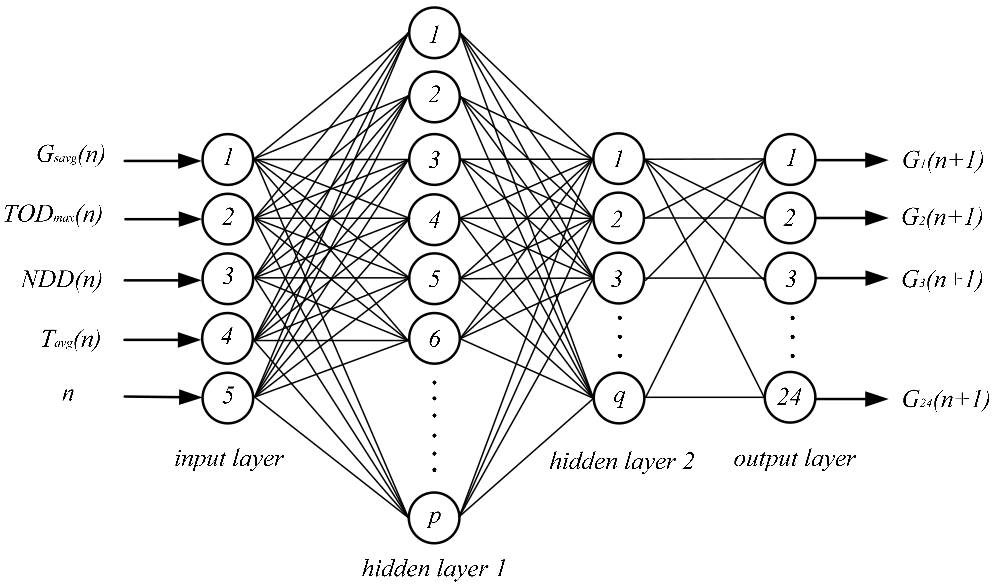
\includegraphics[scale=0.35]{pictures/ER4.png}
  \caption{Modelo de pronóstico ANN utilizando parámetros de características estadísticas.} 
  \label{fig:er4}
\end{figure}
\newpage

\cite{sai2014estimation} señala dos enfoques para obtener radiación neta diaria utilizando los productos de Kalpana VHRR y Oceansat OCM2 mediante el manejo de  la radiación 
de onda larga resultante del flujo de ondas entrantes y salientes, este resultado es computarizado usando la ecuación de Stefan Boltzmann para 
corregir la humedad y la nubosidad,  también se realiza un enfoque basado en la estimación mediante la computación de un cielo despejado con el 
flujo de ondas cortas de radiación que permiten obtener una radiación neta

\begin{figure}[htb]
  \centering 
  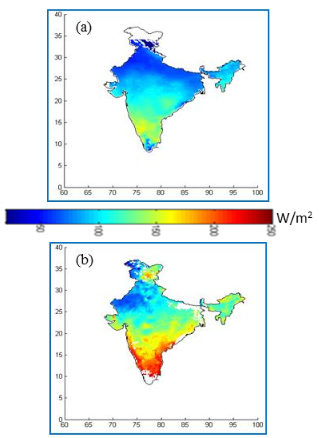
\includegraphics[scale=0.7]{pictures/ER6.png}
  \caption{ Radiación superficial diaria neta de productos de Kalpana VHRR y Oceansat OCM2.} 
  \label{fig:er6}
\end{figure}
\newpage
\cite{mas2011aplicaciones},\cite{ garcia2011evaluacion} generan información de cobertura de suelo, y los métodos que permiten obtener más detalle conservando una fiabilidad 
aceptable sobre la región del Tancítaro, Michoacán y comprende bosques templados y tropicales secos, pastizales y áreas 
de cultivos. Enfocan el estudio en índices de vegetación mediante compuestos espectrales de 8 días e imágenes de reflectancia diarias que 
fueron evaluados por medio de dos metodologías; la máxima verosimilitud y redes neuronales, en cada una de estas se incorporaron 
dos tipos de datos auxiliares. Los resultados muestran que es posible obtener mapas confiables a partir de estos datos de baja resolución 
si se usan categorías generales.

\begin{figure}[htb]
  \centering 
  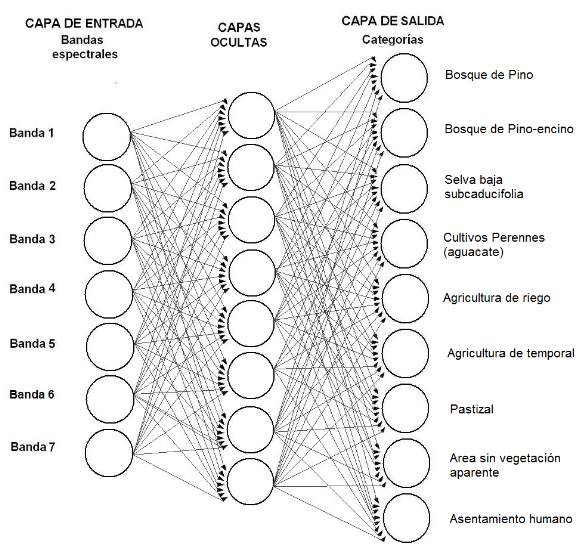
\includegraphics[scale=0.6]{pictures/ER7.png}
  \caption{ Red Neuronal perceptrón multicapa para clasificar una imagen de siete bandas en nueve categorías} 
  \label{fig:er7}
\end{figure}
\newpage
\textbf{\cite{kim2008estimation}} destaca la correlación existente entre la radiación solar incidente en la superficie terrestre y la radiación solar reflejada al espacio; Adicionalmente 
realiza un estudio comparativo en el análisis de  imágenes satelitales MODIS respecto a imágenes satelitales provenientes de SRB, Earth Observing System
(EOS) y Tropical Rainfall Measuring Mission (TRMM), en este estudio se destaca los métodos para estimar la radiación neta obtenida de ondas cortas 
medidas en la superficie.

\newpage
\textbf{\cite{alvarezprocesamiento}} prueban diferentes algorítmos para la detección de aerosoles sobre la superficie terrestre contempladas dentro de imágenes 
satelitales MODIS, implementación del algorithmo Miller sobre las bandas de infrarojo y adicionalmente se realiza una clasificación de los aerosoles detectado.

\begin{figure}[htb]
  \centering 
  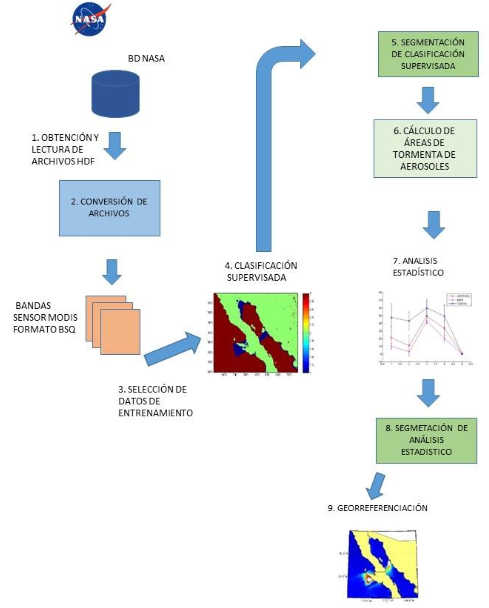
\includegraphics[scale=0.65]{pictures/ER8.png}
  \caption{ Detección de Aerosoles a partir de imágenes satelitales MODIS} 
  \label{fig:er8}
\end{figure}
\newpage
\cite{hashimoto2012prediction} calcula la caída de potencial y fluctuaciones en la generación de energía a partir del seguimiento tridimensional de nubes y su impacto sobre paneles solares.
\begin{figure}[htb]
  \centering 
  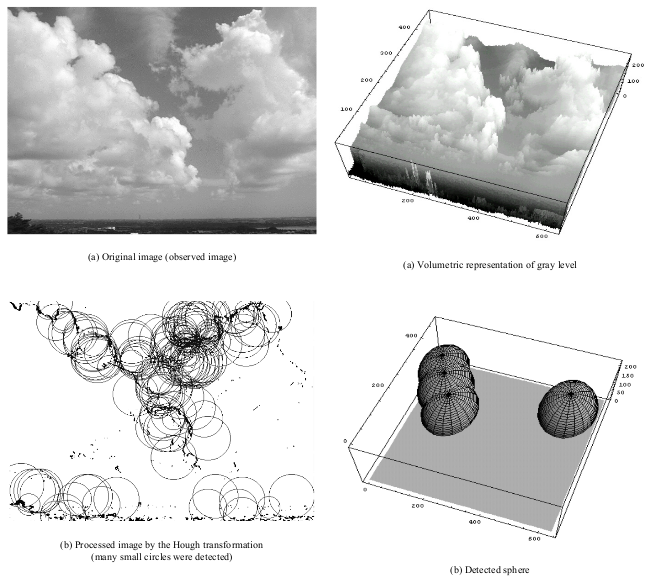
\includegraphics[scale=0.65]{pictures/ER5.png}
  \label{fig:er5}
\end{figure}

 
\chapter{METODOLOGÍA}
Para poder cumplir todos los objetivos de la investigación, inicialmente se realizó la apropiación de 
conocimiento correspondiente con la temática y se definió el marco conceptual sobre el cual se iba a realizar el proyecto. Como primer paso 
fué importante entender la problemática que se pretende solucionar, identificar los recursos necesarios para el estudio y fijar las metas 
que se pretende alcanzar, las actividades mas relevantes empleadas en la investigación son detalladas a continuación:

\section{Identificar y Adquirir Imágenes Satelitales}
Se realiza el estudio de las imágenes satelitales más pertinentes para obtener la información, para la elección se tiene 
en cuenta 4 factores importantes \textit{resolución espacial}, \textit{resolución espectral}, \textit{resolución radiométrica} 
y \textit{resolución temporal} de la imágen satelital; Las imágenes de LandSat 7 son generadas cada 16 dias y permiten adquirir
datos de 8 bandas espectrales con una resolución de 15m por pixel para la banda 6 y 30m por pixel para las 7 bandas restantes, 
estas bandas tienen la capacidad de detectar diferentes indicadores para vegetación, reflectancia, temperatura, precipitación, 
nubosidad, etc. Por otra parte, las imágenes satelitales MODIS adquieren datos de 36 bandas espectrales con las cuales ofrece 
el producto MOD09GA con una resolución espacial aproximada de 500x500m en cada pixel, estos productos son generados diariamente 
y están diseñado para medir la reflectancia de la superficie terrestre\cite{mod09gadetails}\cite{modisweb}, MOD09GA 
presenta 7 banadas que tienen relación directa con la delimitación de territorios, tipos de vegetación, incidencia de aerosoles, 
temperatura y reflectancia la cual está relacionada con la propiedad reflectiva de la vegetación y los aerosoles; mediante la propiedad 
reflectiva de la vegetación se pretende realizar una estimación para la radiación solar que se irrádia en una superficie.



\textbf{Descarga de imágenes Satelitales}

Las imágenes satelitales de MODIS están ubicadas en una grilla senosoidal de aproximadamente 10x10 grados cada sección como lo muestra la 
figura~\ref{fig:gridmodis}. Esta grilla cuenta con un índice vertical y un índice horizontal que permiten ubicar la imagen satelital en un 
área determinada; el territorio colombiano se encuentra ubicado en la columna 10 (h10) en la fila 8 (v8) como lo muestra la 
figura~\ref{fig:colombiagridmodis}, estos 2 índices son necesarios para realizar la descarga de todas las imágenes satelitales comprendidas 
entre el año 2005 y 2015 para posteriormente construir la serie de tiempo de radiación solar. El gestor de descargas utilizado en esta 
ocasión es PyModis\cite{pymodisworkwithMODIS}, herramienta que permite la creación de scripts para gestionar las descargas, cambio de formato, 
procesamiento y reproyección de una imágen satelital a un sistema de coordenadas espaciales determinado.
\begin{figure}[htb]
  \centering 
  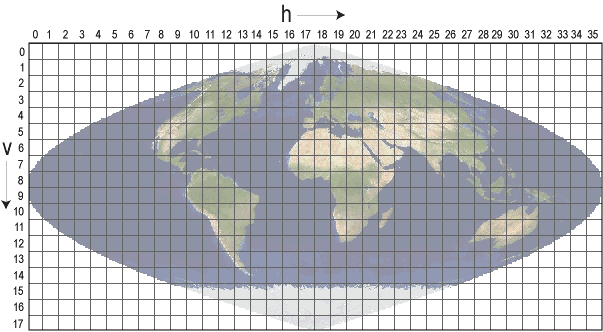
\includegraphics[scale=0.5]{pictures/MODIS_sinusoidal_grid.png}
  \caption{ Grilla Senosoidal de MODIS} 
  \label{fig:gridmodis}
\end{figure}

\begin{figure}[htb]
  \centering 
  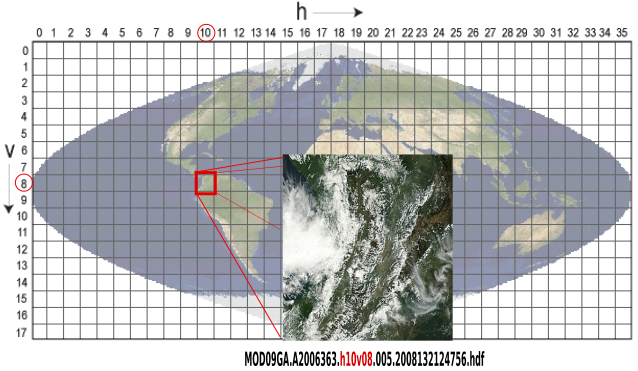
\includegraphics[scale=0.5]{pictures/mipc.png}
  \caption{ Ubicación del territorio colombiano en grilla senosoidal de MODIS} 
  \label{fig:colombiagridmodis}
\end{figure}
Para el caso del sensor MODIS el territorio colombiano y sus 32 departamentos se encuentra ubicado dentro de una sola imágen satelital, por este motivo 
solo se realizó la descarga diaria de una imágen durante los 11 años establecidos.

Por otra parte, las imágenes satelitales de LandSat 7 están ordenadas en una grilla de menor tamaño en comparación con la grilla de MODIS, para ubicar 
una imágen satelital en LandSat 7 se debe tener en cuenta PATH y ROW de las imágenes que logren la cobertura de una región definida como lo muestra 
la figura~\ref{fig:gridlandsat}, EarthExplorer\footnote{\url{http://earthexplorer.usgs.gov/}} permite identificar de manera sencilla las imágenes 
satelitales necesarias para la cobertura de un territorio.
\begin{figure}[htb]
  \centering 
  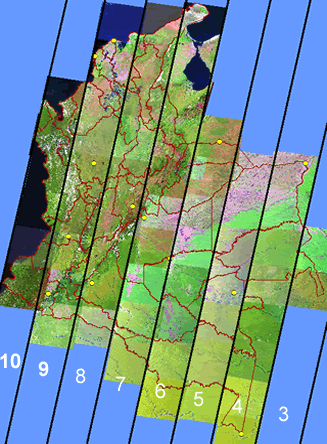
\includegraphics[scale=0.4]{pictures/pc.png}
  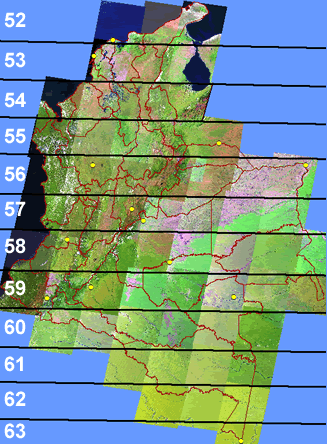
\includegraphics[scale=0.4]{pictures/rc.png}
  \caption{Path y Row de la Grilla sensor LandSat en Colombia - Fuente UNODC Colombia} 
  \label{fig:gridlandsat}
\end{figure}

Para el caso particular del departamento de Nariño, se logra una cobertura del territorio con 5 imágenes satelitales de LandSat 7 correspondientes a 
la lista de paths:rows (9:59), (9:60), (10:58), (10:59), (11:59) como lo muestra la figura~\ref{fig:nl7}.
\begin{figure}[htb]
  \centering 
  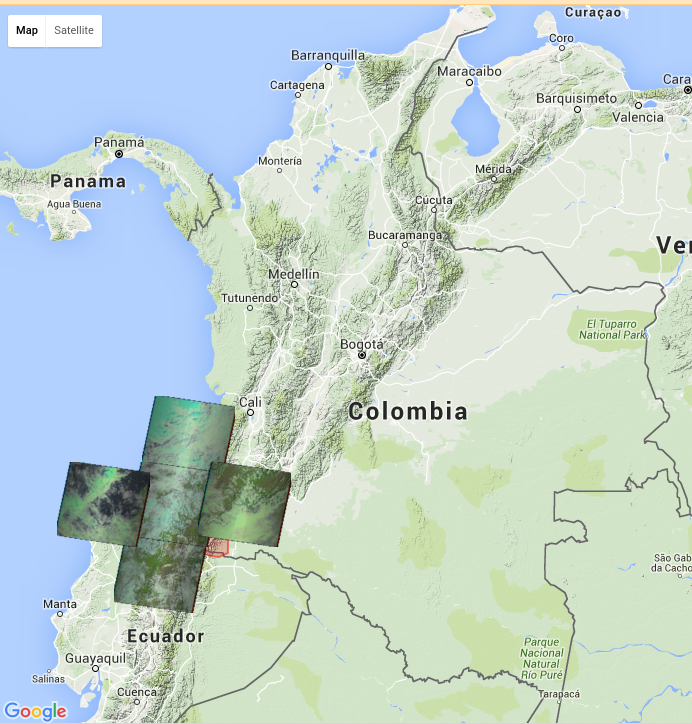
\includegraphics[scale=0.4]{pictures/nl7.png}
  \caption{Paths y Rows necesarios para la cobertura del territorio Nariñense.} 
  \label{fig:nl7}
\end{figure}

Actualmente existe software especializado en manejo de imágenes satelitales; gsutil\footnote{\url{https://cloud.google.com/storage/docs/gsutil}} 
dedicado explícitamente para la descarga de imágenes satelitales LandSat y pyModis\footnote{\url{http://pymodis.fem-environment.eu/}} que facilita 
la descarga y procesamiento a gran cantidad de imágenes satelitales proveniente del sensor MODIS. Para almacenar la información necesaria para 
la estimación de radiación solar sobre el departamento de Nariño se trabajó de forma independiente la manipulación de las imágenes LandSat y 
las imágenes de MODIS. 
\newpage
\section{Procesar y Almacenar Información}

Para el caso de MODIS se desarrolló un script dedicado al manejo de aproximadamente 3.500 imágenes satelitales MOD09GA, mediante el script se convierte 
el formato científico original de la imágen satelital(HDF) en un formato de imágenes de mapa de bits(TIFF) reproyectando el sistema de coordenadas 
espaciales original a  EPSG:3857, se utiliza EPSG:3857 por la simplicidad en cálculos, interpolación, aproximación y manejo en BD. Posterior a la conversión 
de formato y reproyección, se realizó un recorte a la imágen satelital en el que se abarque el territorio de Nariño y se proceda a recorrer las 7 bandas en 
formato TIFF obtenidas del producto MOD09GA, a continuación se almacenan muestras de reflectancia con referencia geográfica a cada 450 metros como lo muestra 
la figura~\ref{fig:dbmodis} y se aplíca el filtro de nubes según las especificaciones de las bandas\cite{bandMODISspecification}.
\begin{figure}[htb]
  \centering 
  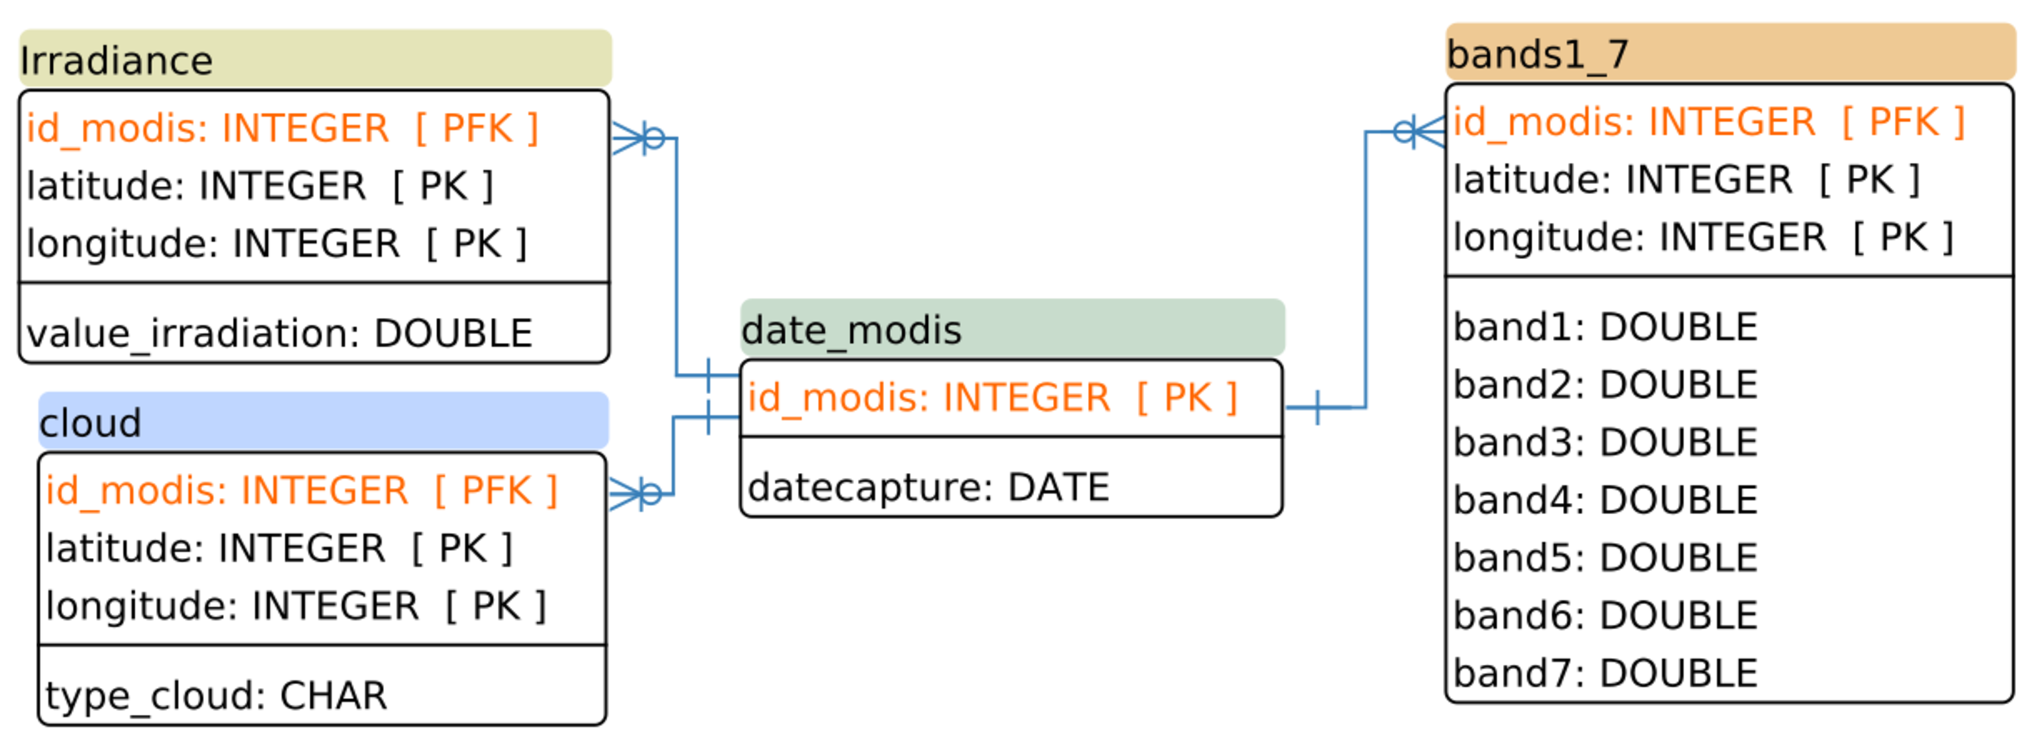
\includegraphics[scale=0.4]{pictures/bdmodis.pdf}
  \caption{Esquema BD para almacenamiento de imágenes satelitales MOD09GA.} 
  \label{fig:dbmodis}
\end{figure}
\newpage
Las imágenes provenientes del sensor LandSat 7 ofrecen 8 bandas que se encuentran compresas y en formato TIFF, para manipular este tipo de imágenes
se tiene en cuenta la reproyección del sistema de coordenadas espaciales original a  EPSG:3857 al igual que se lo realizo con las bandas de MOD09GA, 
para lograr la cobertura del departamento de Nariño es necesario la unión de 5 imágenes satelitales ver figura~\ref{fig:nl7u} y~\ref{fig:nl7}, luego se 
procede a realizar el recorte de la imagen satelital usando el croquis del departamento de Nariño ver figura~\ref{fig:nl7c}.
\begin{figure}[htb]
  \centering 
  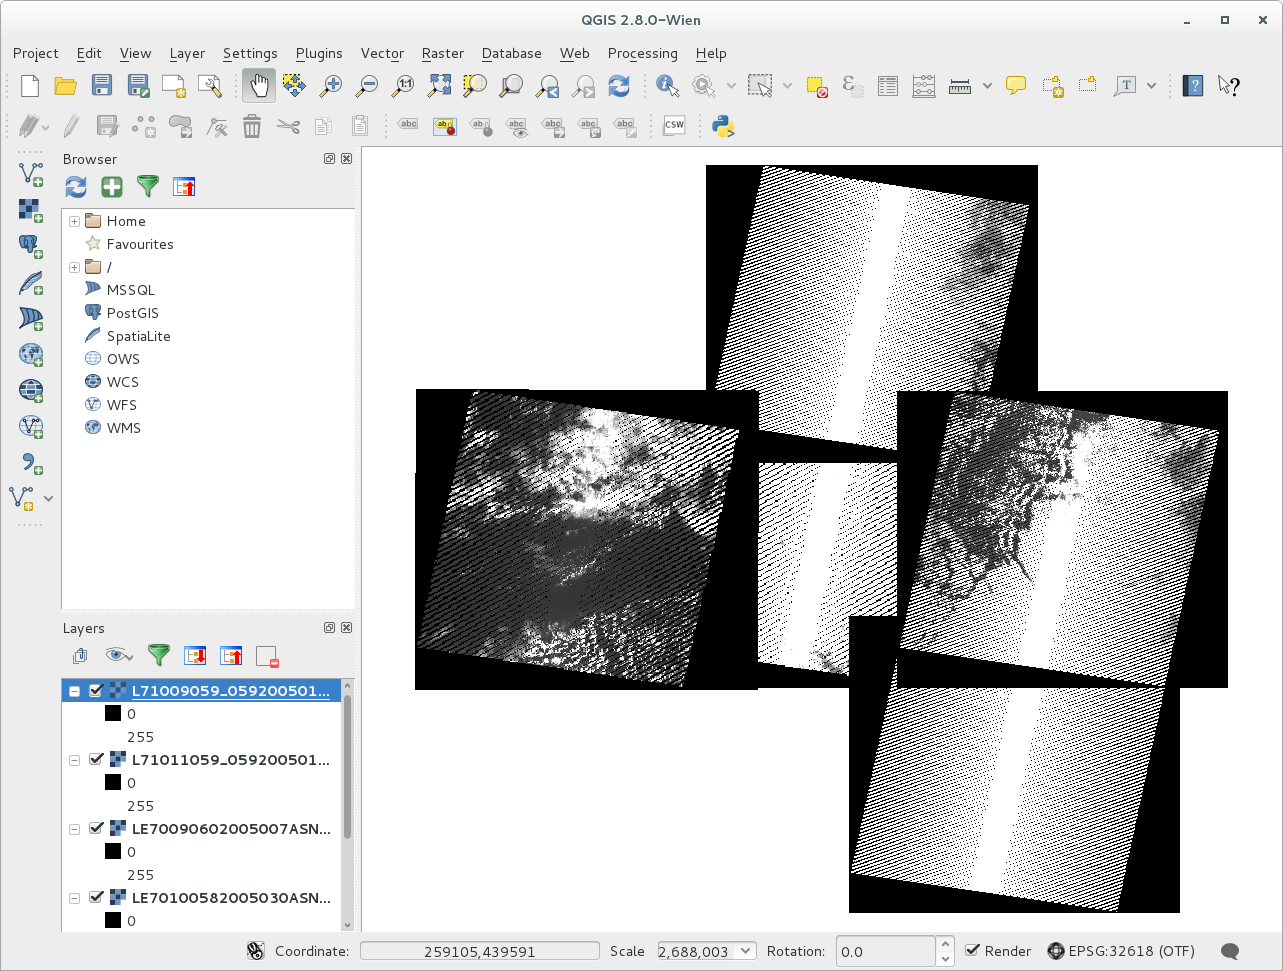
\includegraphics[scale=0.15]{pictures/cut1.png}
  \caption{Imágenes satelitales LandSat para lograr la cobertura del departamento de Nariño.} 
  \label{fig:nl7u}
\end{figure}
\begin{figure}[htb]
  \centering 
  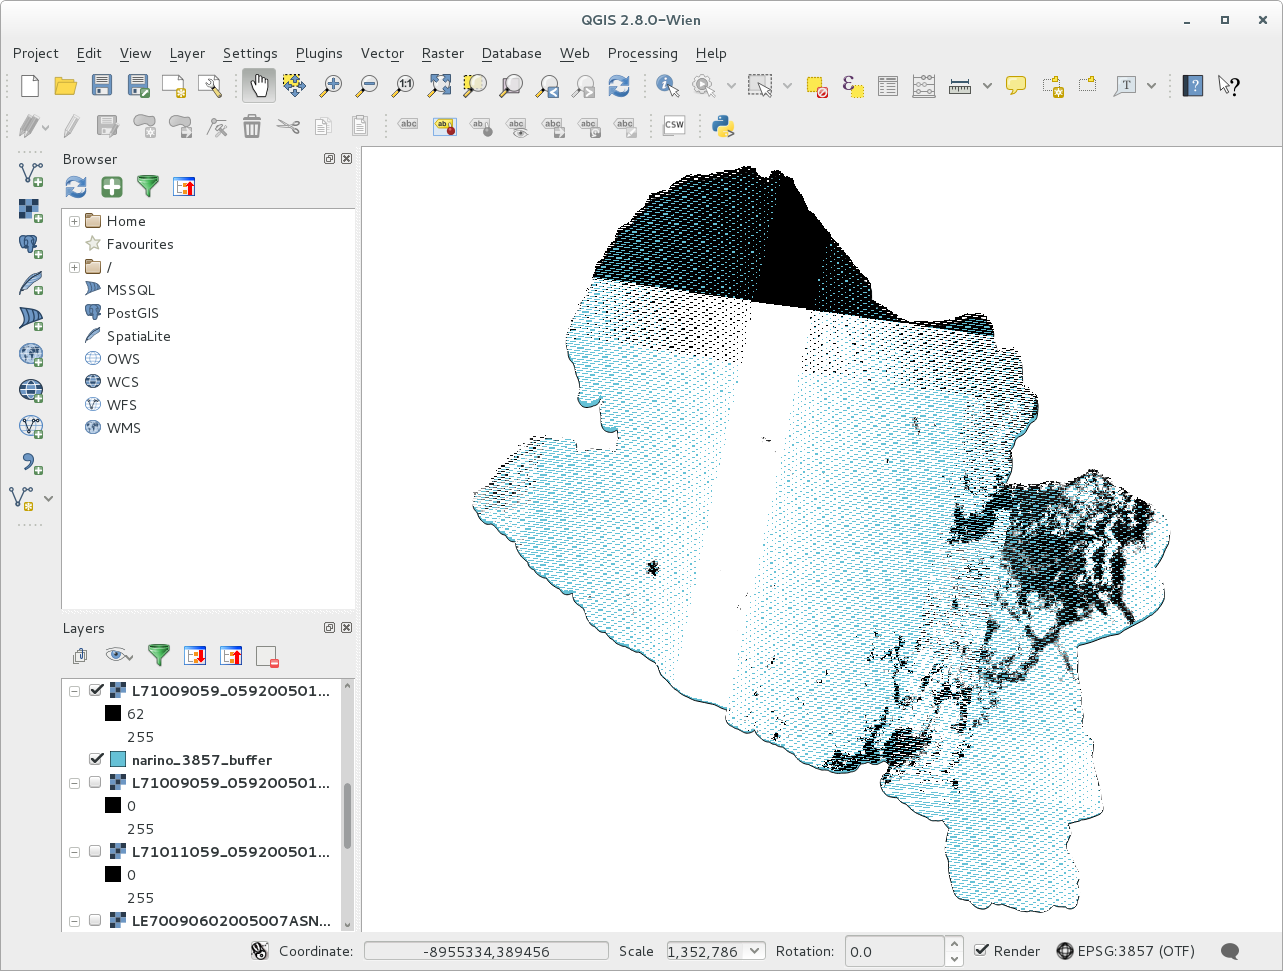
\includegraphics[scale=0.15]{pictures/cut2.png}
  \caption{Recorte de imágenes satelitales LandSat ajustado al territorio Nariñense.} 
  \label{fig:nl7c}
\end{figure}

Una vez terminado la reproyección y recorte de aproximadamente 1.300 imágenes satelitales, se procede a tomar muestras con referencia geográfica del Número 
Digital(DN) la imágen satelital, este número digital indica la escala de gris en la que se encuentra un pixel en determinada banda, esta escala de grises es 
interpretada de diferente forma en cada banda; una vez capturado el DN se procede a calcular la reflectancia, esto se realiza calibrando la muestra mediante 
correcciones atmosferica, estimación la ganancia de las bandas, corrección de ángulo de insidencia del sol, determinación de la distancia de la tierra al sol 
y calculos o correcciones recomendados por LandSat\cite{gasparri2007utilidad}.

La reflectancia obtenida es almacenada en BD ver figura~\ref{fig:dblansat} de igual forma se almacena información  de datos descartados al aplicar un filtro 
para detectar información de nubes, gases, lagos, ciudades, etc.\cite{cea2005mejoras}.
\begin{figure}[htb]
  \centering 
  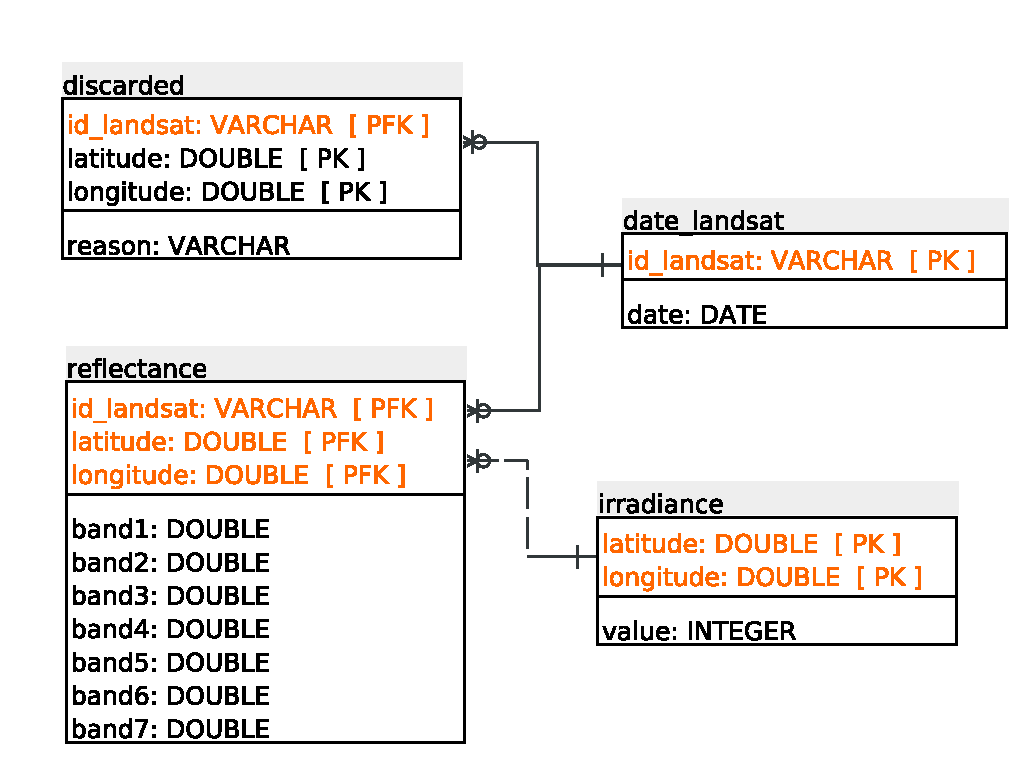
\includegraphics[scale=0.55]{pictures/landsatET.pdf}
  \caption{Esquema BD para almacenamiento de imágen satelital LandSat.} 
  \label{fig:dblansat}
\end{figure}

Finalizado el almacenamiento de las bandas presentes en la imágen satelital, se procede a realizar un muestreo de radiación solar georeferenciado 
proveniente de una fuente confiable de información, en este caso  se seleccionó 500 puntos distribuidos uniformemente sobre el territorio 
de Nariño y se procedió a consultar la información de 3TIER Figura~\ref{fig:m3t} para construir modelos de regresión y 
extrapolar los datos. Para la información referente a nubes se discrimino tres tipos de nubosidad correspondientes a la escala de 
reflectancia\cite{li2003high} según la altura del aerosol.
\begin{figure*}[htb]
  \centering
  \subfigure[Muestras Uniformemente distribuidas en el Departamento de Nariño]{\label{b1} 
  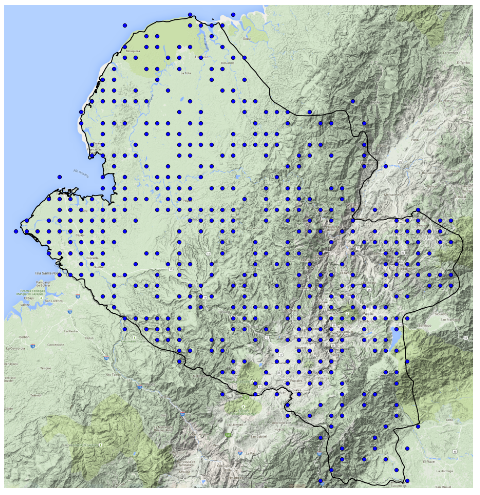
\includegraphics[scale=0.3]{pictures/m3tn.png}}\hspace{5mm}
  \subfigure[Muestras de radiación tomadas manualmente de 3TIER]{\label{b2} 
  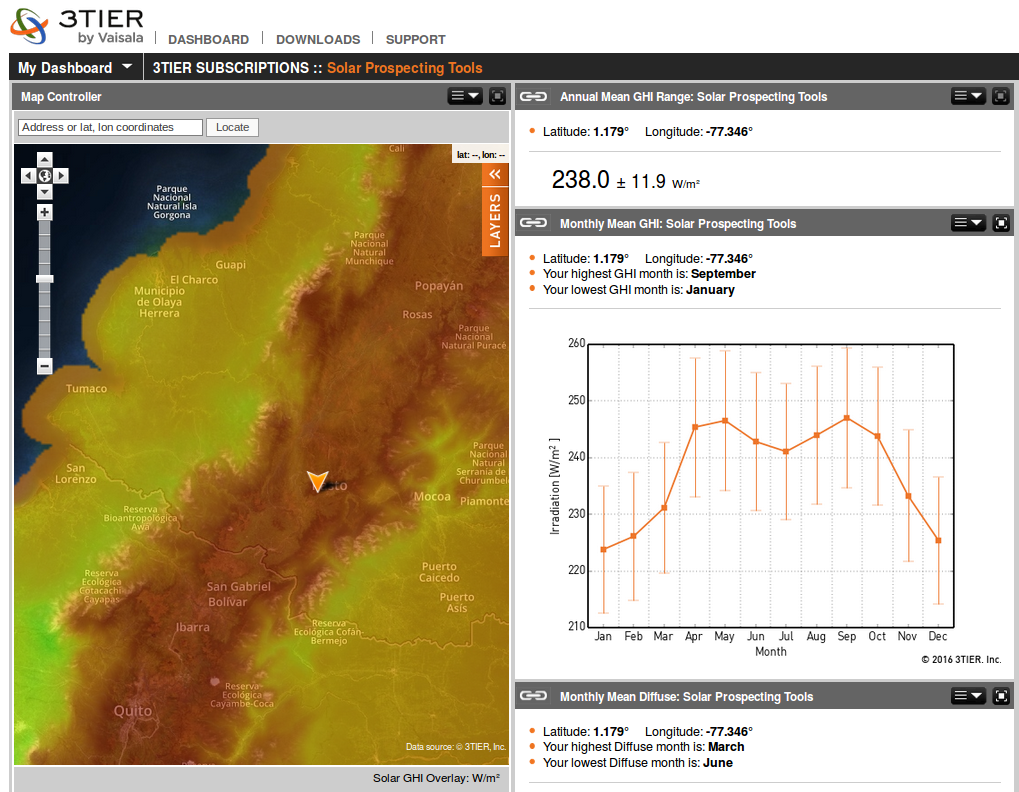
\includegraphics[scale=0.2]{pictures/3t.png}}
  \caption{Muestreo de radiación solar.}
  \label{fig:m3t}
\end{figure*}
\newpage

\section{Selección, Aplicación del Modelo de Regresión y Construcción de Serie de Tiempo}

En base a la información de las muestras recolectadas de 3TIER y la información recolectada de las bandas 1-7 del producto MOD09GA, se desarrolló un script en R 
para construir diferentes modelos de regresión, adicionalmente se evalúa cual es el modelo ideal para ser aplicado a la serie de tiempo y proceder a extrapolar 
los datos de reflectancia a datos de radiación solar, se realizó un análisis con 13 modelos para extrapolar los datos de reflectancia a datos de radiación.

Para la selección del modelo más adecuado se analizó las muestras de reflectancia del producto de MOD09GA y las muestras tomadas de 3TIER, mediante el 
análisis se obtuvo el resultado mostrado en la siguiente tabla ~\ref{tabla:arm}.
\begin{table}[H]
\centering\footnotesize
\begin{tabular}{ >{\arraybackslash}m{2cm} >{\arraybackslash}m{2cm} >{\arraybackslash}m{1.5cm} >{\arraybackslash}m{1.5cm} >{\arraybackslash}m{1.5cm} >{\arraybackslash}m{1.5cm} >{\arraybackslash}m{1.5cm}}
\hline
\textbf{Modelo}& \textbf{SAE} & \textbf{MAE} & \textbf{RAE} & \textbf{RMSE} & \textbf{COR} & $R^2$ \\
\hline \hline
ctree & 1360.88975 & 9.13349 & 60.07076 & 13.06545 & 0.64264 & 0.41299 \\
\hline
rpart & 1373.21922 & 9.21624 & 60.61499 & 14.14182 & 0.60074 & 0.36089 \\
\hline
kknn & 920.48535 & 6.17775 & 40.63096 & 10.31934 & 0.79280 & 0.62854 \\
\hline
mlp & 485.60361 & 3.25908 & 21.43493 & 4.51435 & 0.96284 & 0.92705 \\
\hline
\textbf{mlpe} & \textbf{443.11836} & \textbf{2.97395} & \textbf{19.55960} & \textbf{3.97730} & \textbf{0.97157} & \textbf{0.94394} \\
\hline
ksvm & 823.63424 & 5.52775 & 36.35587 & 8.12712 & 0.87861 & 0.77195 \\
\hline
randomForest & 1159.07988 & 7.77906 & 51.16271 & 11.04659 & 0.75129 & 0.56444 \\
\hline
mr & 597.58282 & 4.01062 & 26.37778 & 5.36391 & 0.94694 & 0.89670 \\
\hline
mars & 618.82261 & 4.15317 & 27.31532 & 5.47634 & 0.94475 & 0.89255  \\
\hline
cubist & 597.29188 & 4.00867 & 26.36494 & 5.36508 & 0.94688 & 0.89658 \\
\hline
pcr & 597.58282 & 4.01062 & 26.37778 & 5.36391 & 0.94694 & 0.89670 \\
\hline
plsr & 597.58282 & 4.01062 & 26.37778 & 5.36391 & 0.94694 & 0.89670 \\
\hline
cppls & 597.58282 & 4.01062 & 26.37778 & 5.36391 & 0.94694 & 0.89670 \\
\hline
\end{tabular}
\caption{\scriptsize{Análisis de modelos de Regresión aplicados a datos de reflectancia de 7 bandas de MOD09GA.}}
\label{tabla:arm}
\end{table}

Para encontrar el modelo más adecuado se realizó un análisis a los datos de reflectancia de LandSat y las muestras tomadas de 3TIER, los resultados se observan 
en la siguiente tabla~\ref{tabla:arl}.
\begin{table}[H]
\centering\footnotesize
\begin{tabular}{ >{\arraybackslash}m{2cm} >{\arraybackslash}m{2cm} >{\arraybackslash}m{1.5cm} >{\arraybackslash}m{1.5cm} >{\arraybackslash}m{1.5cm} >{\arraybackslash}m{1.5cm} >{\arraybackslash}m{1.5cm}}
\hline
\textbf{Modelo}& \textbf{SAE} & \textbf{MAE} & \textbf{RAE} & \textbf{RMSE} & \textbf{COR} & $R^2$ \\
\hline \hline
ctree & 771.66185 & 5.32181 & 33.37397 & 8.89544 & 0.85991 & 0.73945 \\
\hline
rpart & 819.97501 & 5.65500 & 35.46349 & 9.23174 & 0.84774 & 0.71865 \\
\hline
kknn & 583.36151 & 4.02318 & 25.23008 & 6.19161 & 0.93584 & 0.87580 \\
\hline
mlp & 558.43603 & 3.85128 & 24.15206 & 5.49114 & 0.94968 & 0.90189 \\
\hline
\textbf{mlpe} & \textbf{461.93253} & \textbf{3.18574} & \textbf{19.97834} & \textbf{4.73616} & \textbf{0.96292} & \textbf{0.92721} \\
\hline
ksvm & 574.76656 & 3.96391 & 24.85835 & 5.71528 & 0.94664 & 0.89613 \\
\hline
randomForest & 663.70528 & 4.57728 & 28.70490 & 6.89480 & 0.92117 & 0.84856 \\
\hline
mr & 752.19550 & 5.18756 & 32.53206 & 6.75745 & 0.92222 & 0.85049 \\
\hline
mars & 680.67053 & 4.69428 & 29.43864 & 6.34212 & 0.93186 & 0.86837 \\
\hline
cubist & 538.20590 & 3.71176 & 23.27712 & 6.34056 & 0.93141 & 0.86752 \\
\hline
pcr & 748.89239 & 5.16478 & 32.38920 & 6.76538 & 0.92208 & 0.85023 \\
\hline
plsr & 748.89239 & 5.16478 & 32.38920 & 6.76538 & 0.92208 & 0.85023 \\
\hline
cppls & 748.89239 & 5.16478 & 32.38920 & 6.76538 & 0.92208 & 0.85023 \\
\hline
\end{tabular}
\caption{\scriptsize{Análisis de modelos de Regresión aplicados a datos de reflectancia de 8 bandas de LandSat.}}
\label{tabla:arl}
\end{table}

%Las metricas evaluadas indican 
%\scriptsize{
%\texttt{\noindent
%\hspace{7ex}$R^2\to $Coeficiente de determinación\\
%\phantom{x}\hspace{6ex}$COR\to $Correlación\\
%\phantom{x}\hspace{6ex}$RMSE\to $Raíz del error cuadrático medio\\
%\phantom{x}\hspace{6ex}$RAE\to $Error absoluto relativo\\
%\phantom{x}\hspace{6ex}$MAE\to $Error medio absoluto\\
%\phantom{x}\hspace{6ex}$RMSE\to $Raíz del error cuadrático medio\\
%\phantom{x}\hspace{6ex}$SAE\to $Suma (Error Absoluto)/(Desviacion)\\
%}}
Según las métricas SAE, MAE, RAE, RMSE, COR y $R^2$ evaluadas en los 13 modelos \cite{ASH:2013:Online}, se logra concluir que el modelo más óptimo para extrapolar 
los datos de radiación es ``mlpe''–multilayer perceptron ensemble, mlpe es un modelo implementado en R que se basa en una red neuronal artificial con la capacidad 
de detectar características en los datos de la bandas de las imágenes satelitales LandSat y el producto MOD09GA, posteriormente el modelo se encarga de asociarlos 
a un valor objetivo y determinar las métricas de relación más comunes. Al realizar el análisis de los modelos se logra construir los todos modelos de regresión que 
son utilizados para extrapolar los datos, en este caso se procede a construir la serie de tiempo de radiación solar mediante la aplicación del modelo más óptimo; 
mlpe se encarga de evaluar los datos de reflectancia contenidos en las 7 bandas de MOD09GA y asocia un resultado de radiación que es almacenado en BD, de la misma 
forma analiza las 8 bandas de LandSat almacenados en la relación Radiance de la BD ver figura~\ref{fig:mlpe} y entrega como resultado un valor de radiación que es 
almacenado en BD.

\begin{figure}[htb]
  \centering 
  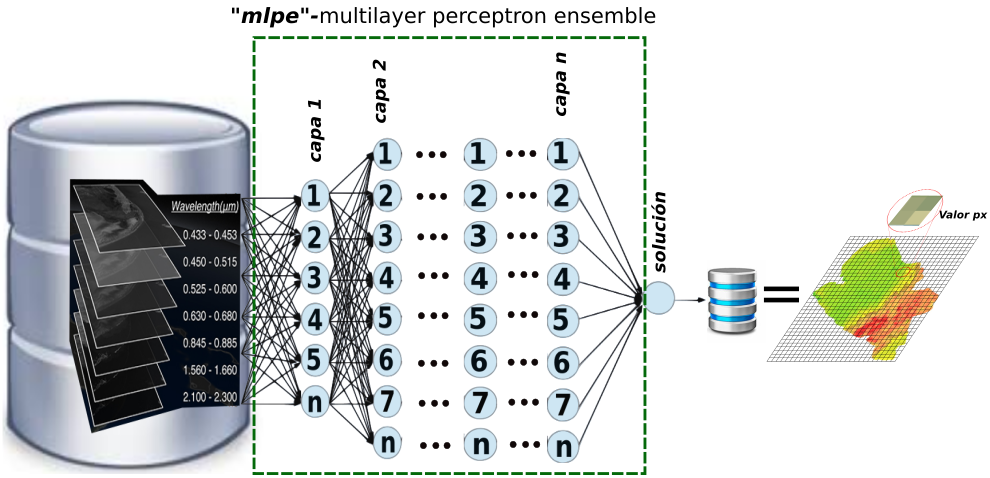
\includegraphics[scale=0.43]{pictures/mlpe.png}
  \caption{Proceso construcción serie de tiempo radiación solar a partir de imágenes satelitales LandSat y MODIS} 
  \label{fig:mlpe}
\end{figure}


\section{Mapas de Radiación Aplicando Interpolación Espacial}
 
La manera más adecuada de visualizar la información es mediante la creación de mapas de promedios mensuales, anuales y un promedio general 
de radiación solar sobre el departamento de Nariño. Una vez construida la serie de tiempo, se procede obtener agregados 
mensuales con el objetivo de establecer cual es el mes con más alta o baja radiación solar, el promedio anual es necesario para establecer como es la variación de la 
radiación solar en el transcurso del tiempo y el promedio general permite establecer la radiación solar promedio en Nariño para los 11 años de MODIS o 15 años de 
LandSat. Una vez obtenidos los agregados mensuales y anuales se desarrolló un script en R que permite implementar la interpolación espacial aplicando el método 
kriging mediante el uso de una grilla de 450x450m que indica la resolución del pixel para el mapa de radiación generado, adicionalmente se debe parametrizar 
el sistema de referencia de coordenadas estándar EPSG:3857 y formato GeoTiff para los mapas ver figuras~\ref{fig:g},~\ref{fig:agregadosm}y ~\ref{fig:agregadosa}; 
estos parámetros sirven para cualquier manejo cartográfico o manipulación de los mapas en un SIG.

\begin{figure}[htb]
  \centering 
  \subfigure[Mapa general de radiación solar MODIS]{\label{b1} 
  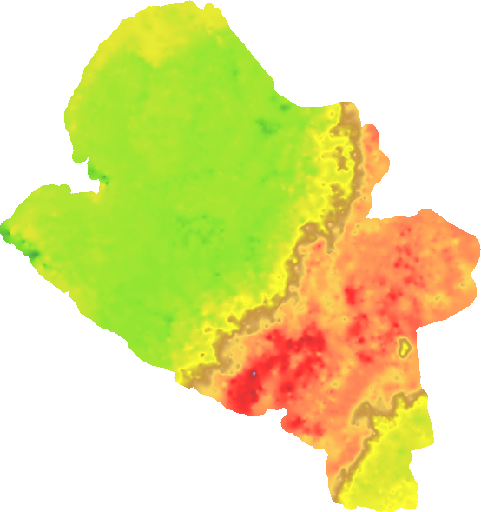
\includegraphics[scale=0.3]{pictures/mapM.png}}\hspace{10mm}
  \subfigure[Mapa general de radiación LandSat]{\label{b2} 
  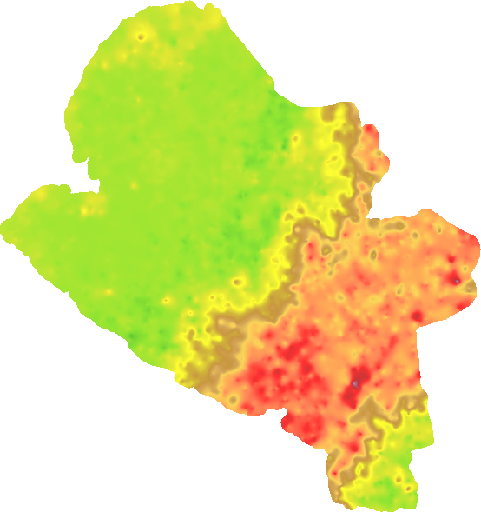
\includegraphics[scale=0.3]{pictures/mapL.png}} 
  \label{fig:g}
  \caption{Promedios de radiación solar}
\end{figure}

En terminos generales el mapa de radiación de MODIS tiene mayor número de muestras en comparación con los mapas de LandSat, pero se puede observar
similaridad en la imágenes al representar la estimación de radiación solar sobre el departamento de Nariño.

\begin{figure}[htb]
  \centering
  \subfigure[Mapas mensuales de radiación solar MODIS]{\label{b3} 
  \includegraphics[scale=0.3]{pictures/months.pdf}}\hspace{5mm}
  \subfigure[Mapa mensuales de radiación solar LandSat]{\label{b4} 
  \includegraphics[scale=0.25]{pictures/monthsL.pdf}}
  \label{fig:agregadosm}
  \caption{Promedios Mensuales}
\end{figure}

\begin{figure}[htb]
  \centering
  \subfigure[Mapas anuales de radiación solar MODIS (2005-2015)]{\label{b5} 
  \includegraphics[scale=0.29]{pictures/years.pdf}}\hspace{4mm}
  \subfigure[Mapas anuales de radiación solar LandSat (2000-2014)]{\label{b6} 
  \includegraphics[scale=0.27]{pictures/yearsL.pdf}}
  \label{fig:agregadosa}
  \caption{Promedios Anuales}
\end{figure}

Los mapas en formato GeoTiff son almacenados en BD para mayor simplicidad en el manejo de información y reportes, de forma complementaria son presentados en la 
plataforma GEOAlternar \footnote{\url{http://geoalternar.udenar.edu.co}} ver figura~\ref{fig:plataforma} permitiendo visualizar mapas, datos de promedios mensuales, 
datos de promedios anuales, descargar datos, generar reportes y buscar información de radiación solar, eólica, biomasa e hídrica presente en cualquier punto dentro 
del territorio Nariñense.
\begin{figure}[tbp]
  \centering 
  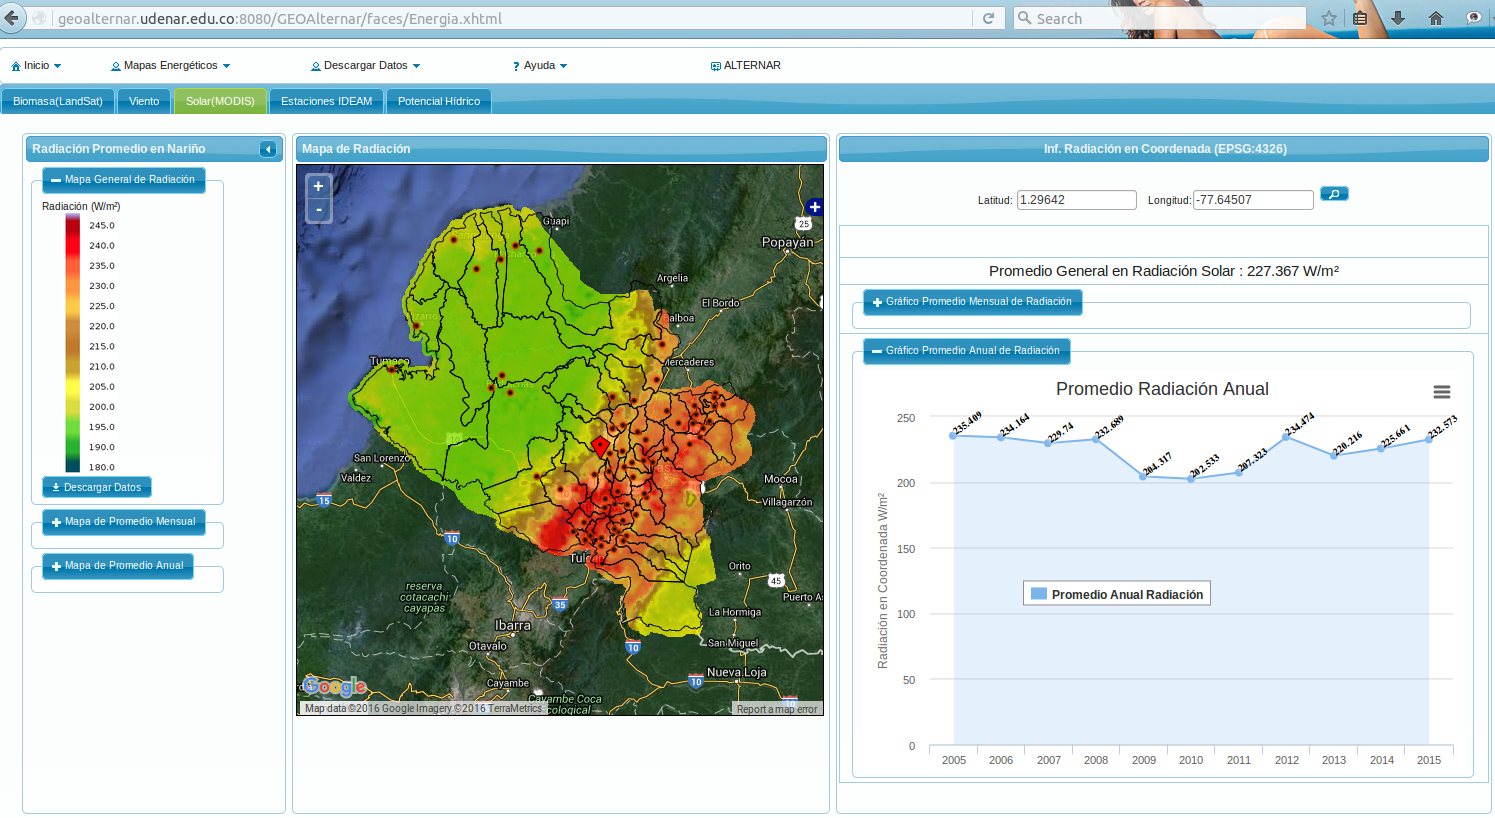
\includegraphics[scale=0.3]{pictures/plataforma.png}
  \caption{ Plataforma GEOAlternar- mapas energéticos del departamento de Nariño}
  \label{fig:plataforma}
\end{figure}

La gran ventaja de crear los mapas de radiación se ve reflejada en la fácil identificación de zonas con potencial de radiación solar, esta información es importante 
para futuras instalaciones de plantas energéticas a base de paneles solares o energía térmica, adicionalmente se puede contemplar el comportamiento mes a mes o año 
tras año de la radiación solar en una área específica.


\section{Detección de Patrones Secuenciales}

La detección de patrones secuenciales se las realizó utilizando la serie de tiempo construida anteriormente mediante los datos del sensor MODIS y el modelo mlpe.
Se aplicó un proceso de minería de datos a la serie de tiempo de radiación solar con el objetivo de extraer información de eventos frecuentes mediante 
la identificación de patrones secuenciales. Para este proceso se cuenta con las relaciones Irradiance y Datemodis ver figura~\ref{fig:insumos} con un historial 
de 11 años de datos que abarcan aproximadamente 340 millones de registros, también se realizó la selección de los 300 mejores puntos 
ver figura~\ref{fig:insumos} con mayor radiación solar dentro del departamento de Nariño, luego se sometió los registro 
histórico de radiación al algoritmo de LCM secuencial. 
\begin{figure*}[tb]
  \centering
  \subfigure[Mejores 300 puntos de radiación solar dentro del departamento de Nariño]{\label{b1} 
  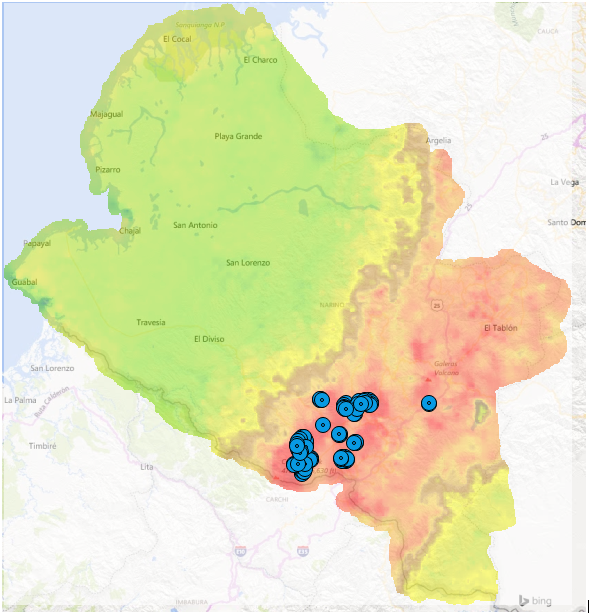
\includegraphics[scale=0.35]{pictures/300bp.png}}
  \subfigure[Relaciones para identificación de patrones secuenciales]{\label{b2} 
  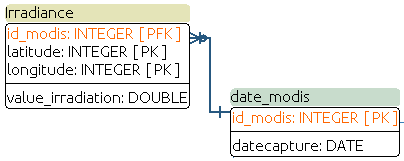
\includegraphics[scale=0.6]{pictures/bdpatterns.png}}
  \caption{Insumos para identificación de patrones secuenciales}
  \label{fig:insumos}
\end{figure*}
\newpage
La detección de patrones se realizó mediante el uso del algorítmo LCM secuencial\cite{uno2005lcm} el cual permite enumerar la frecuencia de acontecimientos 
presentes en una serie de tiempo; el algorítmo LCM secuencial cuenta con las funcionalidades necesarias para detección de patrones secuenciales por lo que 
es necesario establecer los parámetros para realiza la extracción de la información, para el proceso de minería se desarrolló un script en Python que permite 
ejecutar LCM secuencial y aplicarlo a la serie de tiempo de radiación solar utilizado los siguientes parámetros:
\begin{itemize}
 \item Serie de tiempo de muestra de radiación solar.
 \item Generación de 8 bines los cuales permiten discriminar la radiación como se muestra en la tabla~\ref{tabla:patrones}.
 \item Ventana de 30 dias para evaluar la ocurrencia de acontecimientos.
 \item Soporte de 90\%  para las transacciones.
\end{itemize}

\begin{table}[H]
\centering
\begin{tabular}{ >{\centering\arraybackslash}m{2cm} >{\centering\arraybackslash}m{5cm} >{\centering\arraybackslash}m{5cm}}
\hline
Bin & Rango radiación solar& Representación \\
\hline \hline
1 & (x<195.985) - 195.985 & 
\includegraphics[width=5mm]{pictures/suns/so1.png} \\
\hline
2 & 195.985 - 196.496 & 
\includegraphics[width=5mm]{pictures/suns/so2.png} \\
\hline
3 & 196.496 - 197.047 & 
\includegraphics[width=5mm]{pictures/suns/so3.png} \\
\hline
4 & 197.047 - 199.124 & 
\includegraphics[width=5mm]{pictures/suns/so4.png} \\
\hline
5 & 199.124 - 205.954 & 
\includegraphics[width=5mm]{pictures/suns/so5.png} \\
\hline
6 & 205.954 - 228.426 & 
\includegraphics[width=5mm]{pictures/suns/so6.png} \\
\hline
7 & 228.426 - 233.534 & 
\includegraphics[width=5mm]{pictures/suns/so7.png} \\
\hline
8 & 233.534 - (x>233.534) & 
\includegraphics[width=5mm]{pictures/suns/so8.png} \\
\hline
\end{tabular}
\caption{Bines utilizados en la detección y representación de patrones secuenciales.}
\label{tabla:patrones}
\end{table}

Se implementó el algorítmo incluyendo los parámetros correspondientes, el pseudo-código base propuesto se contempla en Algorítmo ~\ref{alg:patt}.

\begin{algorithm}
  \renewcommand{\algorithmicrequire}{\textbf{Input:}}
  \renewcommand{\algorithmicensure}{\textbf{Output:}}
  \caption{Identificación de Patrones Secuenciales}
  \label{alg:patt}
  \algsetup{indent=2em}
  \footnotesize
  \begin{algorithmic}[1]
    \REQUIRE {BD Seie de Tiempo Radiación}
    \ENSURE {Patrones de Radiación Solar}
    \STATE $ListaPatrones \leftarrow \emptyset$
    \FOR { $SerieTiempoMuestraReflectancia_{lat,lon} \in$ BD Serie de Tiempo Radiación}
      \STATE $Soporte \leftarrow $90\%
      \STATE $Bines \leftarrow $[Tabla ~\ref{tabla:patrones}]
      \FOR {$Ventana \in SerieTiempoMReflectancia_{lat,lon}$}
	  \STATE {Patron $\leftarrow$ Aplicar $LCM\_seq(_{MReflectancia(_{lat,lon}), Bines,Soporte})$  \tiny{ LCM Algorithm \cite{uno2005lcm}}}
	  \STATE {FP $\leftarrow Patron_{Frecuente}$ }
	  \STATE {DP $\leftarrow Patron_{Diferente}$ }
	  \STATE {TP $\leftarrow Patron_{Tamaño}$ }
	\ENDFOR
      \STATE $ListaPatrones \leftarrow FP,DP,TP$ 
      \STATE $ALmacenar Patron DB$ 
    \ENDFOR
  \end{algorithmic}
\end{algorithm}

Los resultados obtenidos son almacenados en BD ver figura~\ref{fig:bdp} para posteriormente proceder al análisis y visualización. Tal y como muestra la figura~\ref{fig:bdp}
se creó la relación ``patrones por día'' que presenta 8 atributos donde los más relevantes para identificar patrones son detallados a continuación.

\texttt{\noindent
\phantom{x}\hspace{5ex}$latitude-longitude\to $\footnotesize Ubicación geográfica en el sistema de coordenadas EPSG:3857 \\
\phantom{x}\hspace{6ex}$pattern\to $ \footnotesize Representa la detección de un conjunto de bines del la tabla ~\ref{tabla:patrones}. \\
\phantom{x}\hspace{6ex}$len\_pattern\to $\footnotesize Indica el número consecutivo de dias de la ocurrencia de un evento.\\
\phantom{x}\hspace{6ex}$frecuency\to $\footnotesize Indica la frecuencia del patrón detectado.\\
\phantom{x}\hspace{6ex}$solar\to $\footnotesize Representa el conjunto de bines en el rango de la escala solar~\ref{tabla:patrones}.\\
\phantom{x}\hspace{6ex}$diff\_solar\to $\footnotesize Registra los tipos de bines que hay en el patrón.\\
}

Para la representación visual de los patrones detectados en los 300 mejores puntos de radiación, se desarrolló un script para generar un archivo kml que permite
visualizar la ubicación geográfica, dias presentes y frecuencia del patrón como lo muestra la figura~\ref{fig:visualizarpatron}, el archivo es desplegado sobre la plataforma google-earth.

\begin{figure}[htbp]
  \centering 
  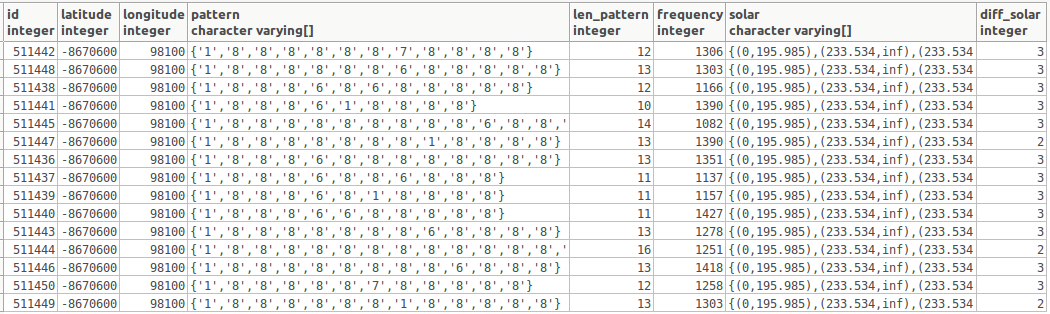
\includegraphics[scale=0.40]{pictures/bdp.png}
  \caption{Base de datos resultado de aplicación LCM secuencial}
  \label{fig:bdp}
  \centering
  \subfigure[Ubicación geográfica de los patrones de radiación en departamento de Nariño]{\label{b1} 
  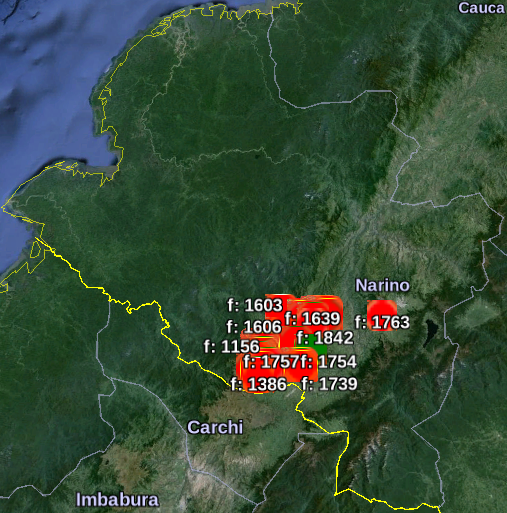
\includegraphics[scale=0.27]{pictures/ugp.png}}
  \subfigure[Acercamiento a zona con patrones de radiación solar]{\label{b2} 
  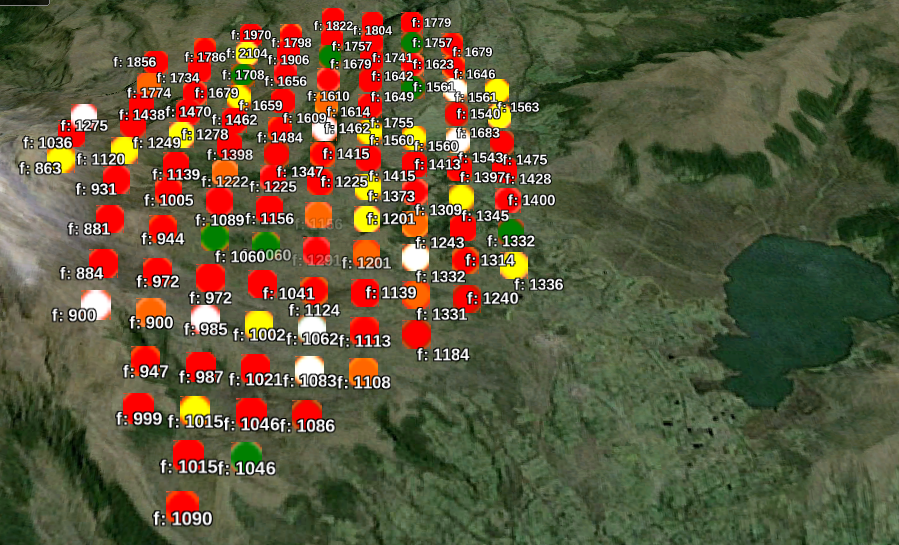
\includegraphics[scale=0.25]{pictures/apg.png}}
  \subfigure[Detalle de patrón de radiación solar]{\label{b3} 
  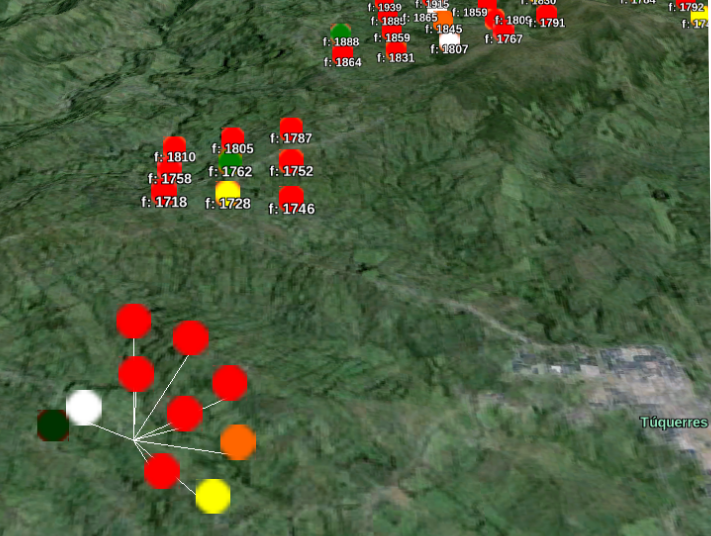
\includegraphics[scale=0.25]{pictures/pdg.png}}
  \caption{Visualización de patrones de radiación solar}
  \label{fig:visualizarpatron}
\end{figure}

Los patrones detectados anteriormente permiten establecer un periodo de de tiempo con presencia de radiación solar constante, en este periodo se puede aprovechar 
al máximo las plantas solares debido a que se puede garantizar una óptima radiación solar por un numero determinado de dias.
\newpage

\section{Comportamiento de Nubes}

El comportamiento de las nubes está estrechamente ligado a la producción de energía a base de paneles de radiación solar
o energía térmica, por este motivo fué necesario construir un registro histórico referente a la presencia de nubes, 
este registro permite evidenciar la presencia de aerosoles sobre el departamento de Nariño, haciendo
posible la identificación de la presencia de de nubosidad en una zona con potencial de radiación solar. La identificación de nubes se realizó 
mediante filtros aplicados a las muestras de reflectancia, el filtro se implemento teniendo en cuenta el tratamiento y las recomendaciones necesarias 
que se deben dar a las bandas de la imagen satelital\cite{modisweb}\cite{bandMODISspecification}\cite{cea2005mejoras}.

Para identificar el comportamiento de las nubes se utilizó el registro histórico con el objetivo de establecer la probabilidad 
para la presencia de nubes en una zona determinada. Como primera medida se construyó una BD donde se almacena la 
probabilidad de la presencia de nubes en un punto determinado para construir la BD fué necesario realizar un conteo de los dias
del mes en los que se presentó nubes en cada punto dentro del departamento de Nariño, posteriormente se agrupo mensual y anualmente para calcular 
la probabilidad y establecer un promedio para la presencia de nubes en un punto determinado como se muestra en la figura~\ref{fig:nuvesmes}. 

\begin{figure}[htb]
  \centering 
  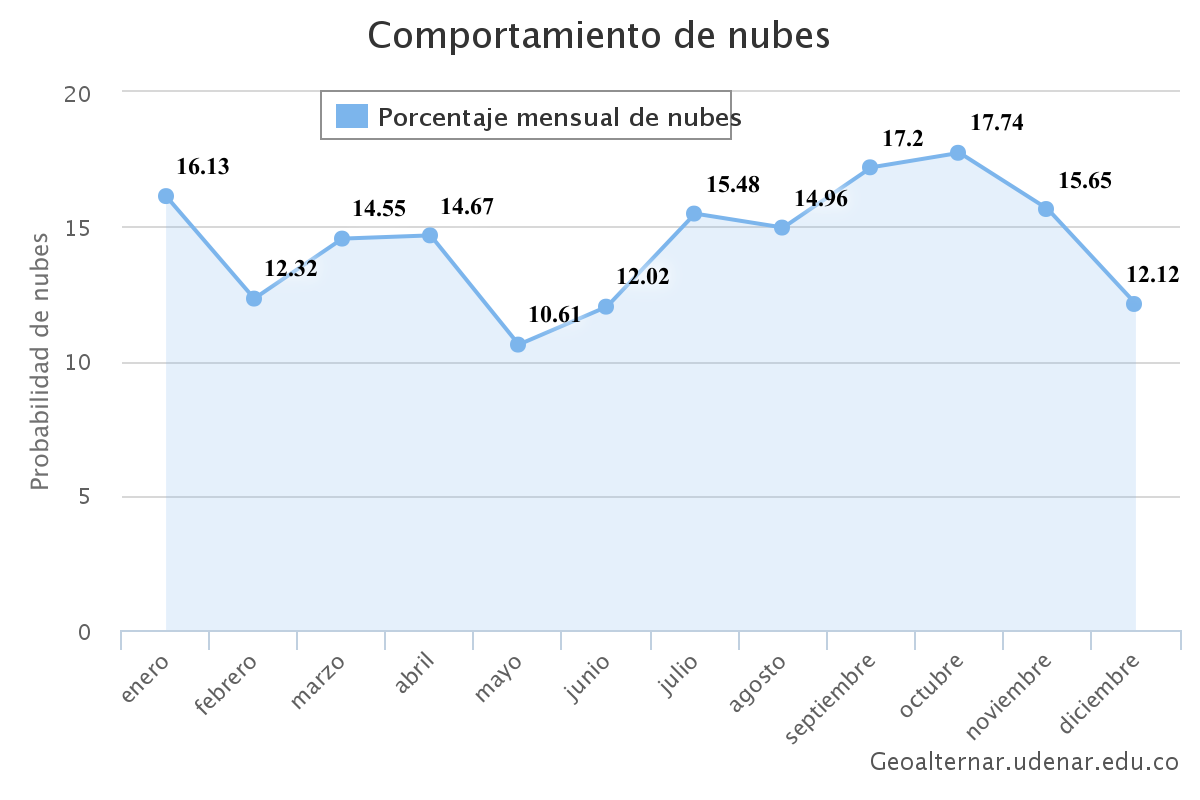
\includegraphics[scale=0.3]{pictures/nubesmes.png}
  \caption{Comportamiento mensual de nubes en un punto específico}
  \label{fig:nuvesmes}
\end{figure}

Los promedios mensuales permiten establecer como es el comportamiento de las nubes en el tiempo para un
punto específico dentro del territorio Nariñense, con esta información se hace posible preveer la presencia  
nubosidad sobre plantas de energía solar en un periodo determinado y tomar medidas adicionales para mitigar los efectos, 
por ejemplo, si se logra determinar en que zonas hay periodos de abundante radiación pero también existe una época donde se presenta gran nubosidad;
esta información permite contrarrestar los periodos de baja radiación mediante el uso de generadores de energía con fuentes alternativas como eólica, 
hídrica o biomasa.


\chapter{Validación de Información con Estaciones Activas}


Actualmente en el departamento de Nariño se han instalado alrededor de 25 estaciones con la capacidad de reportar datos radiación solar, viento, 
precipitación, temperatura y humedad del aire Figura~\ref{fig:stationsalternar}; de las 25 estaciones instaladas se realizó la selección de 11 
estaciones Figura~\ref{fig:stationstested}, esta decisión fué aplicada por inconvenientes en las estaciones como tiempos cortos de reporte de estaciones, debido 
a que muchas estaciones fueron instaladas a finales del año 2015, este corto tiempo de reporte no permite medir con gran certeza la relación entre 
la serie de tiempo construida y los reportes de las estaciones que fueron instaladas hace pocos meses, otros factores que provocaron que se descartaran varias 
estaciones son los errores en el reporte de datos ocasionados por fallas en la calibración de los dispositivos, interrupciones en reporte 
de información, diferencia en tipo de dispositivo y factores exógenos que inciden de forma importante en el reporte de datos. 
\begin{figure}[htb]
  \centering 
  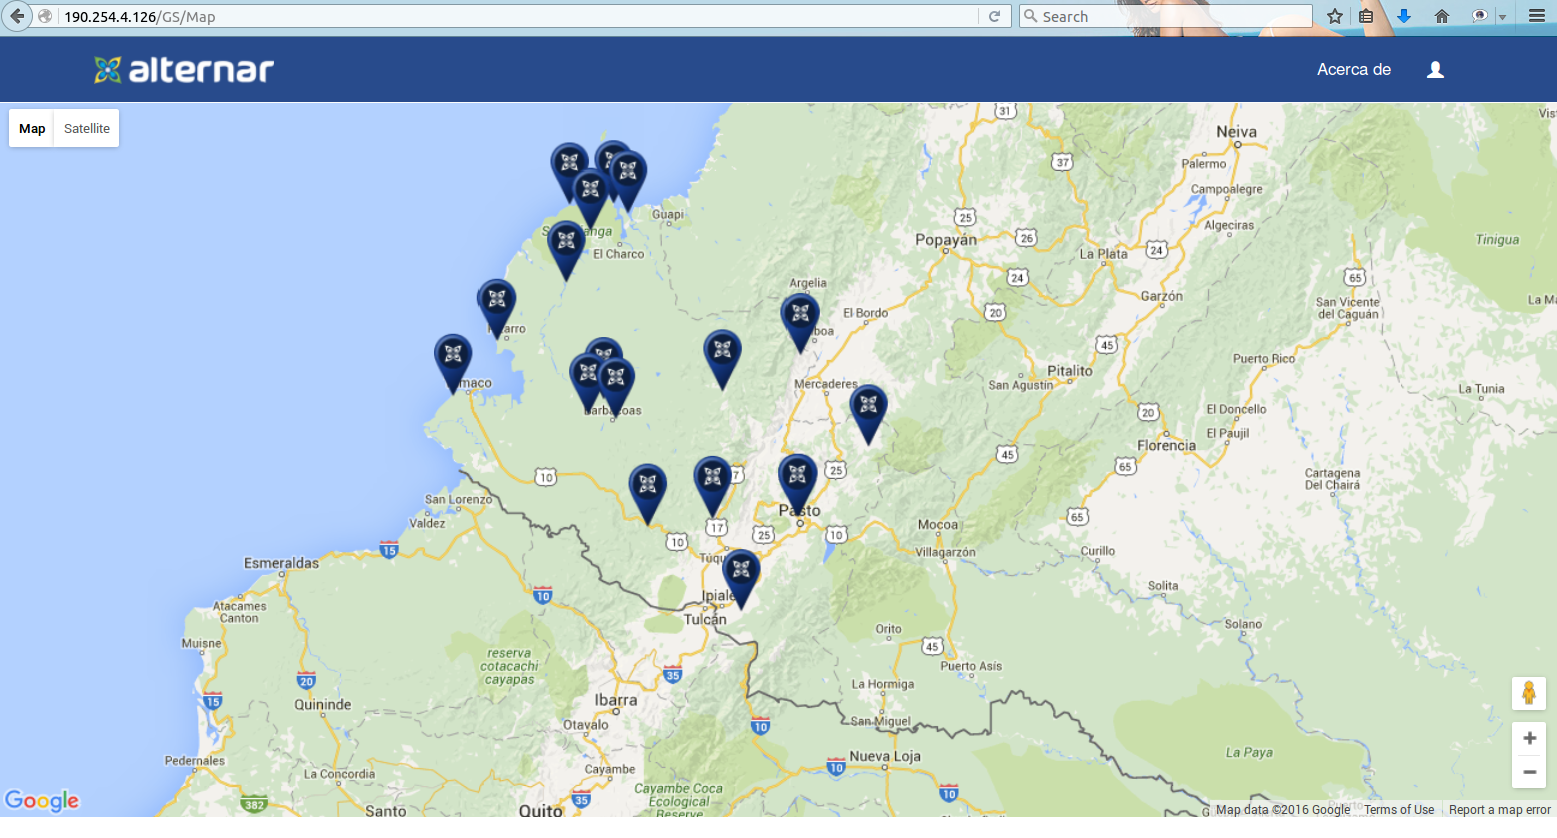
\includegraphics[scale=0.27]{pictures/stationsalternar.png}
  \caption{Plataforma de reporte y ubicación de estaciones del proyecto Alternar}
  \label{fig:stationsalternar}
\end{figure}
\begin{figure}[htb]
  \centering 
  \includegraphics[scale=0.45]{pictures/stationstested.png}
  \caption{Estaciones seleccionadas para proceder a validación de datos de radiación solar}
  \label{fig:stationstested}
\end{figure}
En la validación es necesario gran cantidad de muestras que permitan establecer una mayor certeza en el análisis de los datos reales con los datos de las imágenes
satelitales, por este motivo es importante destacar que las imágenes satelitales MODIS tienen una resolución temporal diaria mientras que las imágenes 
satelitales LandSat tiene una resolución temporal cada 16 dias, por este motivo se descartó para la validación los datos de LandSat.

Al disponer del registro histórico de las 11 estaciones, se procede a realizar la validación de los datos de radiación solar; para el proceso de validación es 
necesario obtener los promedios mensuales de las 11 estaciones y los promedios mensuales de radiación de la serie de tiempo construida ubicando la zona 
correspondiente, los promedios obtenidos permiten establecer una correlación buena entre los datos de radiación solar de las estaciones y los datos de radiación 
solar de MODIS. A continuación se puede observar los resultados obtenidos del análisis realizado a las 11 estaciones con reportes superiores a 5 meses y 
la serie de tiempo de radiación solar obtenida del sensor MODIS.

\begin{table}[H]
\centering
\begin{tabular}{ >{\arraybackslash}m{7cm} >{\centering\arraybackslash}m{5cm} >{\centering\arraybackslash}m{3cm}}
\hline
Estación & Ubicación & $R^2$ \\
\hline \hline
Estación Mosquera& (-78.333333,2.655) & 86,57 \% \\
\hline
Estación Ricaurte & (-77.975833,1.186944) & 90,33 \%\\
\hline
Granja Barbacoas & (-78.18173,1.361483333) & 74,09 \%\\
\hline
Granja Betania & (-77.257028,1.186317) & 84,64 \%\\
\hline
Granja Buesaco & (-77.04079,1.35932) & 76,55 \%\\
\hline
Granja Catambuco & (-77.290397,1.166761) & 60,82 \%\\
\hline
Granja La Cruz & (-76.9640701,1.5955594) & 91,26 \%\\
\hline
Granja Obonuco & (-77.305556,1.193458) & 71,52 \%\\
\hline
Granja Pupiales & (-77.624667,0.867483) & 90,47 \%\\
\hline
Granja San Lorenzo & (-77.219125,1.503858) & 65,11 \%\\
\hline
Granja Santa Barbara & (-77.305544,1.078422) & 81,27 \%\\
\hline
\end{tabular}
\caption{Análisis datos de radiación solar Reporte Estaciones Vs Serie de Tiempo MODIS.}
\label{tabla:validacion}
\end{table}
\chapter{Análisis de Resultados}

Al comparar los resultados obtenidos al construir los mapas de radiación solar de Landsat  con lo de MODIS se puede observar gran similitud,
la manera de establecer relación entre los datos es mediante un análisis de correlación y coeficiente de determinación entre los mapas resultantes 
con los datos de Landsat7 y MODIS. Se tomo los mapas por años del 2005 al 2014  como lo muestra la tabla~\ref{tab:landsatvsmodisanio}, por meses y el 
mapa general ver tabla~\ref{tab:landsatvsmodismes}

Adicionalmente se muestra resultados de datos reales reportados por las estaciones y se los compara con la serie de tiempo construida a partir de imágenes satelitales
MODIS, los resultados obtenidos permiten concluir que la serie de tiempo de radiación solar construida para todo el departamento de Nariño es fiable y puede servir 
como punto de referencia para varios estudios que contemplen la temática.
\begin{table}[H]
\centering
\begin{tabular}{ >{\arraybackslash}m{5cm} >{\centering\arraybackslash}m{3cm}}
\hline
Estación & $R^2$ \\
\hline \hline
Estación Mosquera&  86,57 \% \\
\hline
Estación Ricaurte & 90,33 \%\\
\hline
Granja Barbacoas & 74,09 \%\\
\hline
Granja Betania & 84,64 \%\\
\hline
Granja Buesaco & 76,55 \%\\
\hline
Granja Catambuco & 60,82 \%\\
\hline
Granja La Cruz & 91,26 \%\\
\hline
Granja Obonuco & 71,52 \%\\
\hline
Granja Pupiales & 90,47 \%\\
\hline
Granja San Lorenzo  & 65,11 \%\\
\hline
Granja Santa Barbara & 81,27 \%\\
\hline
\end{tabular}
\caption{Resultado Análisis de Datos para Radiación Solar Reporte Estaciones Vs Serie de Tiempo MODIS.}
\label{tabla:validacione}
\end{table}

\begin{table}[H]
\label{tab:landsatvsmodisanio}
\centering
\scalebox{1}{
\begin{tabular}{c c c}
\toprule
Map &  COR & R2 \\
\midrule
2005 & 0.85594 & 0.73263 \\
\hline
2006 & 0.90754 & 0.82363  \\
\hline
2007 & 0.92884 & 0.86275 \\
\hline
2008 & 0.90594 & 0.82073  \\
\hline
2009 & 0.89443 & 0.80000  \\
\hline
2010 & 0.88594  & 0.78488  \\
\hline
2011 & 0.88233  & 0.77851  \\
\hline
2012 & 0.92056  & 0.84743  \\
\hline
2013 & 0.92982  & 0.86456  \\
\hline
2014 & 0.93167 & 0.86800  \\
\bottomrule
\end{tabular}}
\caption{Análisis Datos Anuales de MODIS vs Landsat 7}
\end{table}

\begin{table}[H]
\label{tab:landsatvsmodismes}
\centering
\scalebox{1}{
\begin{tabular}{c c c}
\toprule
Map &  COR & R2 \\
\midrule
January & 0.89182 & 0.79535 \\
\hline
February & 0.89131 & 0.79444 \\
\hline
March & 0.90943 & 0.82706 \\
\hline
April & 0.90930 & 0.82683 \\
\hline
May & 0.91770 & 0.84218 \\
\hline
June & 0.90244 & 0.81439 \\
\hline
July & 0.90434 & 0.81783 \\
\hline
August & 0.91527 & 0.83772 \\
\hline
September & 0.91810 & 0.84290 \\
\hline
October & 0.92340 & 0.85266 \\
\hline
November & 0.87242 & 0.76111 \\
\hline
December & 0.86934 & 0.75576 \\
\hline
General & 0.94179 & 0.88696 \\
\bottomrule
\end{tabular}}
\caption{Análisis Datos Mensuales de MODIS vs Landsat 7}
\end{table}
\newpage
\chapter{Análisis de Patrón y Nubes en un punto Específico}
Los patrones identificados en la serie de tiempo de los mejores 300 puntos de radiación dentro departamento de Nariño permiten determinar acontecimiento 
frecuentes respecto a los dias en que se presenta mayor o menor radiación solar, por ejemplo para el punto (0.97067,-77.84763) Figura~\ref{fig:pp}, se 
identificó el patrón ['8','1','7','8','6','8','8','8','8','8'] el significado de este patrón esta representado en la tabla ~\ref{tab:pats}, este patrón 
se presentó 1320 veces y permite concluir que de los 10 dias de radiación hay 7 dias en los cuales se presenta radiación superior a 233.5 W/m2 y se puede 
garantizar que este punto es una zona con buena radiación solar, esta información es necesaria para instalar plantas energéticas a base de paneles solares 
siempre que la frecuencia de nubes sea baja.
\begin{figure}[htbp]
  \centering 
  \includegraphics[scale=0.55]{pictures/pp.png}
  \caption{ Plataforma GEOAlternar- mapas energéticos del departamento de Nariño}
  \label{fig:pp}
\end{figure}

\begin{table}[H]
\label{tab:pats}
\centering
\begin{tabular}{>{\centering\arraybackslash}m{2cm} >{\centering\arraybackslash}m{3cm} >{\centering\arraybackslash}m{3cm} >{\centering\arraybackslash}m{5cm}}
\hline
N. Dias & Bin BD(Patrón) &  Color & Rango \\
\hline \hline
1 & 8 & \includegraphics[width=3mm]{pictures/suns/so8.png}  & 233.534 - x>233.534 \\
\hline
2 & 1 & \includegraphics[width=3mm]{pictures/suns/so1.png} & 0 - 195.985\\
\hline
3 & 7 & \includegraphics[width=3mm]{pictures/suns/so7.png} & 228.426 - 233.534 \\
\hline
4 & 8 & \includegraphics[width=3mm]{pictures/suns/so8.png} & 233.534 - x>233.534 \\
\hline
5 & 6 & \includegraphics[width=3mm]{pictures/suns/so6.png} & 205.954 - 228.426 \\
\hline
6 & 8 & \includegraphics[width=3mm]{pictures/suns/so8.png} & 233.534 - x>233.534 \\
\hline
7 & 8 & \includegraphics[width=3mm]{pictures/suns/so8.png} & 233.534 - x>233.534 \\
\hline
8 & 8 & \includegraphics[width=3mm]{pictures/suns/so8.png} & 233.534 - x>233.534 \\
\hline
9 & 8 & \includegraphics[width=3mm]{pictures/suns/so8.png} & 233.534 - x>233.534 \\
\hline
10 & 8 & \includegraphics[width=3mm]{pictures/suns/so8.png} & 233.534 - x>233.534 \\
\hline
\end{tabular}
\caption{Análisis de Patrón en el punto (0.97067,-77.84763)}
\end{table}
La probabilidad de que en el punto (0.97067,-77.84763) se presenten nubes es de 28\% en cuanto al cambio en el tiempo se puede observar en la tabla ~\ref{tab:ncy}
y la tabla ~\ref{tab:ncm}, esta información es muy importante debido a que la presencia constante de nubes termina afectando la producción energética a base
de paneles solares y así poder plantear una solución alternativa para generar energía.
 
\begin{table}[H]
\label{tab:ncy}
\centering
\begin{tabular}{>{\centering\arraybackslash}m{2cm} >{\centering\arraybackslash}m{3cm} }
\hline
Año&Probabilidad \\
\hline\hline
2005&26.1475\% \\
\hline
2006&26.8242\% \\
\hline
2007&31.5918\% \\
\hline
2008&31.1175\% \\
\hline
2009&29.7392\% \\
\hline
2010&26.9092\% \\
\hline
2011&26.0167\% \\
\hline
2012&28.0983\% \\
\hline
2013&28.2908\% \\
\hline
2014&26.67\% \\
\hline
2015&26.9967\% \\
\hline
\end{tabular}
\caption{Nubes en el punto (0.97067,-77.84763)}
\end{table}

\begin{table}[H]
\label{tab:ncm}
\centering
\begin{tabular}{>{\centering\arraybackslash}m{2cm} >{\centering\arraybackslash}m{3cm} }
\hline
Mes& Probabilidad \\
\hline \hline
January&29.676\% \\
\hline
February&31.9309\% \\
\hline
March&35.7782\% \\
\hline
April&25.7582\% \\
\hline
May&27.5673\% \\
\hline
June&31.5164\% \\
\hline
July&28.4464\% \\
\hline
August&26.3918\% \\
\hline
September&27.2718\% \\
\hline
October&23.225\% \\
\hline
November&21.667\% \\
\hline
December&26.129\% \\
\hline
\end{tabular}
\caption{Nubes en el punto (0.97067,-77.84763)}
\end{table}


\chapter{ CONCLUSIONES}
\begin{itemize}
  \item[$*$]Se detectó patrones secuenciales que permiten predecir el comportamiento de fenómenos
    climáticos y su impacto en áreas con potencial de radiación solar dentro del departamento de Nariño.

  \item[$*$]Se construyeron mapas energéticos con el componente solar en el departamento de Nariño,
  usando los sensores Landsat 7 y MODIS, además se construyeron series de tiempo para radiación solar y nubosidad.

  \item[$*$]Las imágenes sateliatles son una gran fuente de información debido a la capacidad de almacenar gran cantidad de registros históricos 
  para diferentes tipos de datos, estos datos poco a poco estan siendo utilizados por organizaciones para determinar características terrestres, 
  fenómenos naturales, condiciones de los mares, características de la vegetación, etc. Por esta razón el uso de imágenes satelitales en la investigación 
  da resultados aproximados y a bajo costo, teniendo en cuenta el costo que puede implicar hacer muestreo en campo. 

  \item[$*$]Como se observó en la validación de los datos resumida en la Tabla~\ref{tabla:validacion} hay un buen porcentaje de fiabilidad para la estimación 
  del radiación solar en las estaciones activas; mediante este hecho se puede plantear que el registro histórico construido para todo el departamento de Nariño, 
  permite tener gran certeza para la toma de desiciones al momento de instalar plantas a base de energía solar en una zona determinada; un resultado agregado al 
  estudio es la identificación de la presencia de nubosidad la cual es fundamental para una óptima generación de energía a base de paneles solares o energía 
  térmica, adicionalmente se puede utilizar los datos de radiación para contemplar los efecto en el tiempo que presenta el sol sobre la vegetación. 

  \item[$*$]La detección de patrones en la serie de tiempo pemite establecer un periodo de tiempo para un óptimo aprovechamiento de las plantas solares 
  debido a que se garantiza un número determinado de dias en los cuales se presentará altas tasas de radiación solar y baja probabilidad de nubes. La metodología 
  para la detección de patrones yá se encuentra establecida para poder ser aplicada a todo el departamento.

  \item[$*$]Las herramientas de software libre son adaptable a las necesidades de los usuarios y productos como LandSat y MODIS de libre descarga presenta estanadres 
  de calidad para los cualquier tipo de estudio.

  \item[$*$]Se realizó una mejora a las estimaciones de radiación presentes en la actualidad, debido a que el reporte generado por el IDEAM no permite observar la 
  diferencia ni cambios de radiacíon sobre el territorio nariñense Figura~\ref{fig:ideamvsmodis}.
  \begin{figure}[htb]
    \centering\subfigure[Información de radiación solar presentada por el IDEAM para el departamento de Nariño]{\label{b1} 
    \includegraphics[scale=0.3]{pictures/narinoideam.png}}
    \centering\subfigure[Información de radiación solar producto de la investigación para el departamento de Nariño]{\label{b2} 
    \includegraphics[scale=0.35]{pictures/general.pdf}}
    \label{fig:ideamvsmodis}
  \end{figure}

  \item[$*$]Se construyó una metodología para la construcción de mapas energéticos con el potencial de radiación solar, el cual se lo puede aplicar en zonas 
  pantropicas de Colombia utilizando imágenes satelitales de los sensores Landsat o MODIS.

  \item[$*$]Además se obtuvieron los siguientes productos:
  \begin{itemize}
    \item 11 mapas solares por año con el sensor MODIS.
    \item 12 mapas solares por mes con imágenes satelitales del sensor MODIS. 
    \item 16 mapas solares por año con el sensor LandSat.
    \item 12 mapas solares por mes con imágenes satelitales del sensor LandSat. 
    \item Serie de tiempo de radiación solar diaria para el departamento de Nariño.
    \item Serie de tiempo nubosidad diaria presente en el departamento de Nariño.
    \item Algoritmo para detección de patrones secuenciales solares.
    \item Algoritmo de detección de patrones secuenciales para nubosidad.
    \item ``GEOAlternar`` Plataforma para la visualización del potencial energético dentro del departamento de Nariño.
    \item Articulo para revista, el cual esta en proceso de evaluacion denominado: Análisis de regresión para el calculo de irradiación solar en el 
    departamento de Nariño (Colombia) utilizando imágenes satelitales Landsat y MODIS.
  \end{itemize}
\end{itemize}

\chapter{TRABAJOS FUTUROS}

La construcción de la serie de tiempo puede ser replicada para todo el territorio colombiano, debido a que se planteó una metodología y actualmente no se cuenta con una
fuente que permita ver a detalle estos tipo de variables climaticas. En la Figura~\ref{fig:colombia} se puede observar el producto MOD09GA y la dimensión con respecto al 
territorio de nariño, con esta observacion se puede concluir que hay facilidad para replicar la metodología hacia los 31 departamentos que componen a Colombia.
\begin{figure}[htb]
  \centering
  \subfigure[Tamaño de la imagen satelital respecto al departamento de Nariño]{\label{b1} 
  \includegraphics[scale=0.3]{pictures/ncm.png}}
  \subfigure[Dimension de territorio colombiano]{\label{b2} 
  \includegraphics[scale=0.35]{pictures/colombia.png}}
  \label{fig:colombia}
\end{figure}

Las imágenes satelitales permiten versatilidad de estudios debido a las propiedades de los sensores con los que cunenta cada satelite, por estas características se puede
enfocar estudios en:

\begin{itemize}
 \item Comportamiento y tipos de vegetación en una región.
 \item Temperatura sobre una región.
 \item Presipitaciones de un territorio.
 \item Estudios de aerosoles sobre una región.
 \item Incendios y efectos sobre las regiones.
 \item Comportamiento de los mares en el tiempo.
 \item Identificación de Biomasa.
 \item Determinar propiedades de la cuencas hídrica.
\end{itemize}






\bibliography{bibliography}
\bibliographystyle{IEEEtran}
\addcontentsline{toc}{chapter}{REFERENCIAS}

\chapter*{ ANEXOS}
\addcontentsline{toc}{chapter}{ANEXOS}

\begin{itemize}
 \item 1
 \item 2
 \item 3
 \item 4í
 
\end{itemize}

\end{document}

